\documentclass[11pt, letterpaper]{article}
\usepackage[utf8]{inputenc}
\addtolength{\oddsidemargin}{-.875in}
\addtolength{\evensidemargin}{-.875in}
\addtolength{\textwidth}{1.75in}
\addtolength{\topmargin}{-.875in}
\addtolength{\textheight}{1.75in}
\usepackage[utf8]{inputenc}
\usepackage{amsmath}
\usepackage{amssymb}
\usepackage{graphicx}
\usepackage[rightcaption]{sidecap}
\usepackage[font=footnotesize,labelfont=bf]{caption}
\usepackage{enumerate}
\usepackage{enumitem}
\usepackage{array}
\newcommand{\tabitem}{~~\llap{\textbullet}~~}
\graphicspath{ {./Figures/} }
\usepackage[margin=5cm]{caption}
\setlength{\parskip}{1em}
\usepackage{pythonhighlight}
% \setlength{\parindent}{0em}
\usepackage{rotating}
\usepackage{hyperref}
\usepackage{gensymb}
\usepackage[english]{babel}
\usepackage{placeins}
\usepackage{listings}
\usepackage[toc,page]{appendix}
\usepackage{placeins}
\usepackage{setspace}
\usepackage{longtable}
\usepackage{listings}
\usepackage{lipsum}
\usepackage{listings}
\usepackage{natbib}
\usepackage{url}
\usepackage{float}
\usepackage{minted}

\usepackage{subcaption}
\usepackage{tocloft}
  \usepackage[compact]{titlesec}
    \titlespacing{\section}{-5pt}{2ex}{1ex}
    \titlespacing{\subsection}{-2pt}{1ex}{0ex}
    \titlespacing{\subsubsection}{0pt}{0.5ex}{0ex}
\usepackage[nodisplayskipstretch]{setspace}
\usepackage[nodisplayskipstretch]{setspace}
\setlength{\belowdisplayskip}{0pt} \setlength{\belowdisplayshortskip}{0pt}
\setlength{\abovedisplayskip}{-15pt} \setlength{\abovedisplayshortskip}{0pt}


\setlength\cftparskip{0pt}

\begin{document}

\begin{titlepage}
    \centering
    \vspace*{\fill}

    \textbf{EXPLORING PERFORMANCE CHARACTERISTICS OF THE CLARK Y AIRFOIL} \\
    
    \textit{Airfoil Lab Report} \\
    AER303 \\
    Aerospace Laboratory 1 \\
    
    Felix Hlady, Rodrigo Salazar, Sritejas Murugan, Sahil Swali\\
    
    Prof. Philippe Lavoie \\
    
    Due Date: 4 December 2023

\begin{abstract}
This report explores the characteristics of a Clark Y airfoil, by measuring the pressure distribution over the surface of the airfoil and in the wake caused by it. Subsequently, this data is used to generate a $C_P$ distribution and velocity profile at various angles of attack, along with a set of $C_L$, $C_M$, and $C_D$ curves against increasing angles of attack. 

Data collected is used to characterize the conditions for stall and the effects such flow separation has on various other forces acting on the airfoil. A wind tunnel with a freestream velocity of 30.31 ± 0.01 m/s was used and it was found that the Clark Y airfoil stalled at $\alpha = 14\degree$. The experimental data measured closely to other data sources for the $C_L$ and $C_D$ Total but varied significantly for the $C_D$ Pressure and $C_M$. Additionally, differences between the pressure and total drag at different flow regimes are discussed.

These results for $C_P$ when compared to theoretical data from XFOIL and other reference experiments showed that our results displayed a high degree of concurrence, lest errors caused due to inconsistencies in the setup. This lab report also delves deeper into exploring the potential reasons for discrepancies and possible steps to mitigate them in the future. 

\end{abstract}

    \vspace*{\fill}
\end{titlepage}

\tableofcontents
\pagenumbering{arabic}
\singlespacing

\newpage

\section{Nomenclature}

\begin{table}[h]
    \centering
    \begin{tabular}{p{5cm}p{11cm}}
        \hline
        Symbol & Name \\
        \hline
        AOA & Angle of Attack\\
        $C_L$ & Coefficient of Lift\\
        $C_D$ & Coefficient of Drag\\
        $C_M$ & Coefficient of Moment\\
        $C_p$ & Coefficient of Pressure\\
        c & Chord Length\\
        $\alpha$ & Angle of Attack\\
        $U_\infty$ & Freestream Velocity\\
        $q_\infty$ & Freestream Dynamic Pressure\\
        N' & Normal Force\\
        TE & Trailing Edge\\
        LE & Leading Edge\\
        A' & Axial Force\\
        $P_u$ & Pressure on the Airfoil Upper Surface\\
        $P_l$ & Pressure on the Airfoil Lower Surface\\
        L' & Lift Force\\
        D' & Drag Force\\
        u & Velocity at a Point After the Airfoil\\
        $\rho$ & Freestream Density\\
        $P_\infty$ & Freestream Pressure\\
        $P_T$ & Total Pressure\\
        $P_S$ & Static Pressure\\

        \hline
    \end{tabular}
    \label{tab:nomenclature}
\end{table}
        
\newpage
    
\section{Introduction}

\subsection{Motivation and Background}

This report explores the characteristics of a Clark Y airfoil at various angles of attacks to characterize pressure distribution and velocity profile, and $C_L$, $C_M$, and $C_D$ curves in near stall conditions. 

\subsection{Concepts and Theory}

\subsubsection{Airfoils \& The Clark Y Airfoil}

An airfoil is the cross-sectional shape of the wing. The wings create lift through a pressure difference between the upper and lower surfaces of the wing: the pressure below the wing is higher than that of the pressure below the wing resulting in a net force upwards i.e. lift \cite{airfoil}. Airfoils, while known for their use on aircraft, also have other uses such as on Formula 1 cars on which they are inverted and used to create down-force. 

The Clark Y airfoil is a specific type of airfoil used in aircraft design such as with model aircraft. The Clark Y airfoil is known for a near-flat lower surface, good overall performance and lift-to-drag ratio at medium Reynolds' number airflows, and a gentle stall \cite{clarky}. This lab will utilize a model of the Clark Y airfoil to explore question about pressure, lift, drag, and moment distributions for the airfoil at various angles of attack. The wake caused by the airfoil will also be studied for further insight. These attributes will subsequently be compared to the characteristic stall angle of the airfoil to discuss implications. 



\subsubsection{Aerodynamic Forces on an Airfoil \& Dimensionless Coefficients}

\begin{figure}[h]
        \centering
        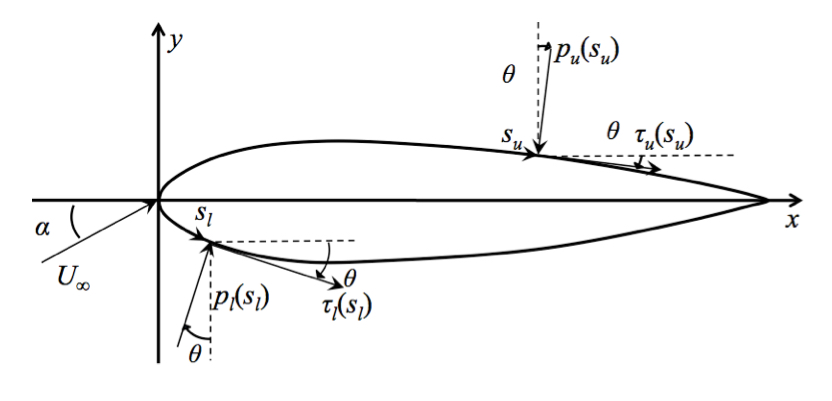
\includegraphics[width=0.5\textwidth]{Images/airfoilpress.jpeg}
        \caption{A diagram showing the pressure and shear stresses on an airfoil.}
        \label{fig:setup_1}
\end{figure}

A fluid exerts forces on an airfoil through pressure differences as well as shear stresses caused by skin friction and viscosity. These result in normal and axial forces ($N'$ and $A'$ respectively) which can be quantified as lift, $L$ and drag, $D$. A moment, $M$, is also produced.

\begin{figure}[h]
        \centering
        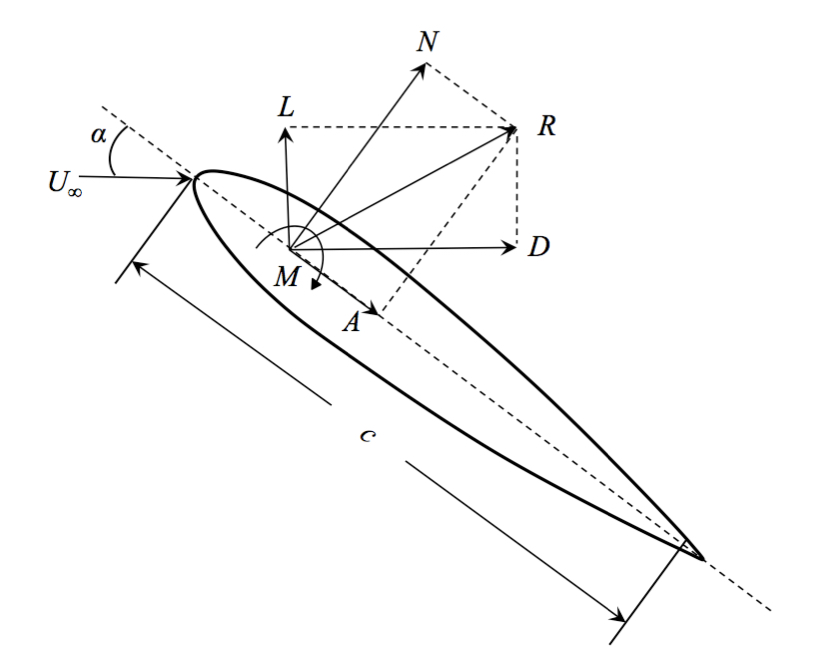
\includegraphics[width=0.5\textwidth]{Images/airfoillandd.jpeg}
        \caption{A diagram showing the forces of lift and drag and moment about the leading edge for an airfoil.}
        \label{fig:setup_2}
\end{figure}

\begin{figure}[h]
        \centering        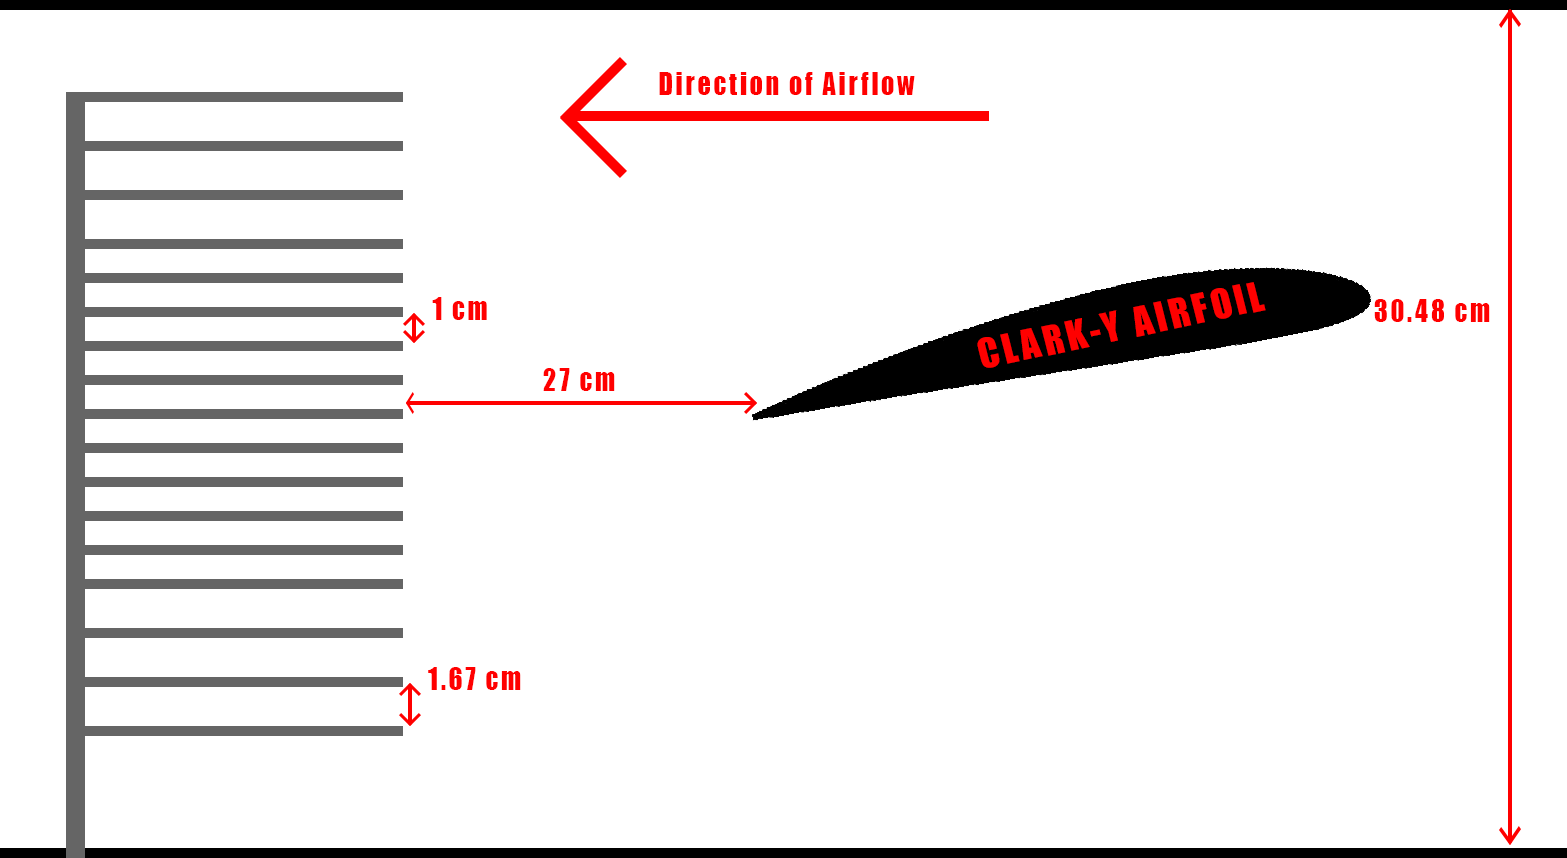
\includegraphics[width=0.8\textwidth]{Images/LAB2.png}
        \caption{A schematic showing the layout of the test section in the subsonic wind tunnel.}
        \label{fig:setup_3}
\end{figure}

The normal force, $N$, and axial force, $A$, as well as moment, $M$, can be calculated by the following formulas, assuming that shear stress is neglected:

\begin{equation}
    N' = \int_{LE}^{TE} -p_u\cos\theta ds_u + \int_{LE}^{TE} p_\ell\cos\theta ds_\ell
    \label{eq:normal_force}
\end{equation}
\begin{equation}
    A' = \int_{LE}^{TE} -p_u\sin\theta ds_u + \int_{LE}^{TE} p_\ell\sin\theta ds_\ell
    \label{eq:axial_force}
\end{equation}
\begin{equation}
M'_{LE} = \int_{LE}^{TE} p_u(x\cos\theta - y\sin\theta) \, ds_u + \int_{LE}^{TE} p_\ell(y\sin\theta - x\cos\theta) \, ds_\ell
\end{equation}

From these, lift, $L$, and drag, $D$ can be found as shown below. Note that $\alpha$ is the angle of attack.

\begin{equation}
L = N \cos(\alpha) - A \sin(\alpha)
\end{equation}
\begin{equation}
D = N \sin(\alpha) + A \cos(\alpha)
\end{equation}

Dimensionless coefficients can be used to for comparison purposes, and are given below. Note that $q_\infty = \frac{1}{2} \cdot \rho_\infty \cdot U_\infty^2$ is the free stream dynamic pressure, where $\rho_\infty$ is the free stream density and $U_\infty$ is the free stream velocity.

\begin{equation}
C_p = \frac{\Delta P}{q_\infty}
\end{equation}

\begin{equation}
C_L = \frac{L'}{q_\infty \cdot c}
\end{equation}

\begin{equation}
C_D = \frac{D'}{q_\infty \cdot c}
\end{equation}

\begin{equation}
C_M = \frac{M'}{q_\infty \cdot c^2}
\end{equation}

\subsubsection{Calculating Total Drag}

The experimental setup used does not measure the shear stress along the airfoil so the above equations can only provide the "pressure drag." The total drag can be obtained from a momentum balance after which the drag per unit span can be found by the following:

\begin{equation}
D = \rho \int_{c}^{d} u \left(U_\infty - u\right) \, dS
\end{equation}

\section{Experimental Setup}

\noindent The following section describes the equipment and procedures used. 

\subsection{Equipment}

This experiment was conducted using an open-return, Eiffel wind tunnel (ELD Model 402B) with a maximum speed of approximately 50 m/s with a 0.61 m long test section with a cross section of 304.8 mm by 304.8 mm. A model Clark Y airfoil was used with 19 pressure taps distributed along the surface and connected via PVC tubes to a pressure measurement device. The coordinates were this airfoil were provided in a .csv file. A table listing the location of the pressure taps numbered clockwise starting from the leading edge tap is given below.

\begin{table}[h]
  \centering
  \caption{Static pressure tap locations}
  \begin{tabular}{cc|cc}
    \hline
    \multicolumn{2}{c|}{Top} & \multicolumn{2}{c}{Bottom} \\
    Tap & $x/c$ & Tap & $x/c$ \\
    \hline
    1 & 0 & 13 & 0.90 \\
    2 & 0.03 & 14 & 0.60 \\
    3 & 0.06 & 15 & 0.40 \\
    4 & 0.10 & 16 & 0.30 \\
    5 & 0.15 & 17 & 0.20 \\
    6 & 0.20 & 18 & 0.10 \\
    7 & 0.30 & 19 & 0.05 \\
    8 & 0.40 \\
    9 & 0.55 \\
    10 & 0.70 \\
    11 & 0.85 \\
    12 & 1.00 \\
    \hline
  \end{tabular}
\end{table}

The wind tunnel speed was monitored by using the outermost ports of the rake to measure the speed of undisturbed air. This rake of total pressure tubes was located at 27 cm downstream of the model's trailing edge, with the relative location of each pressure tube given in the appendix. Pressure differences were measured using a pressure sensor mounted on a mult-channel Scanivalve system. The signal from the pressure transducer connected to the Scanivalve was sampled using a PC via a DAQ and the processed in MATLAB.

\subsection{Procedure}
The following procedures where followed during the lab \footnote{Note: Steps 1-3 were omitted during the lab trial as calibration steps had already been completed by the lab TA or previous groups.}.
\begin{enumerate}
    \item In the initial step, the sampling frequency and sampling time required for precise measurements from the pressure transducer was determined by setting the wind tunnel speed to the specified value and capturing representative samples of the pressure transducer output. Utilizing MATLAB routines, the frequency content and time constant of the signal was analyzed. The sampling time was set to ensure ±1\% accuracy on the transducer signal \cite{lab_manual}.
    \item The pressure transducers were calibrated by developing a calibration curve of the pressure transducer output against the readings from the Betz manometer (prior to lab). These differences were achieved by adjusting the wind tunnel speed \cite{lab_manual}.
    \item A number of angles of attack to investigate for the airfoil was predetermined. 12 angles of attack were chosen with high concentration near the predicted stall angle to better characterize the behaviour of and characteristics of the airflow near stall. The following angles of attack were used: $0\degree$, $4\degree$, $6\degree$, $8\degree$, $9\degree$, $10\degree$, $11\degree$, $12\degree$, $13\degree$, $14\degree$, $15\degree$, and $17\degree$. 
    \item Subsequently, pressure distribution data was collected using the  pressure transducer. Measurements were taken over the airfoil and from the wake rake for all designated angles of attack. When deemed necessary, the wake rake was translated to acquire a more precise wake profile.
\end{enumerate}

\section{Results and Discussion}

\subsection{Pressure over the Airfoil and Velocities in the Wake}

Experimental data collected during the lab was analyzed and processed to develop a measured distribution of pressure coefficient over and under the airfoil. Subsequently, this data was plotted against corresponding theoretical predictions from the XFOIL airfoil analysis software as well as data collected by the University of Illinois at Urbana-Champaign (UIUC) \cite{UIUC}. In addition to this, pressure data collected from the rakes was utilized to approximate the velocity distribution in the wake of the airfoil.

\begin{figure}[h]
  \begin{subfigure}{0.5\textwidth}
    \centering
    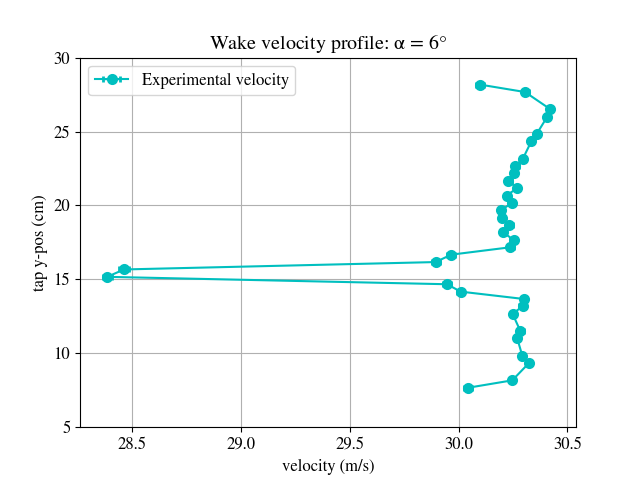
\includegraphics[width=1\linewidth]{Figures/vel-graphs/vel-a6.png}
    \caption{Velocity profile for an alpha of 6\degree.}
    \label{fig:vel-a6}
  \end{subfigure}%
  \begin{subfigure}{0.5\textwidth}
    \centering
    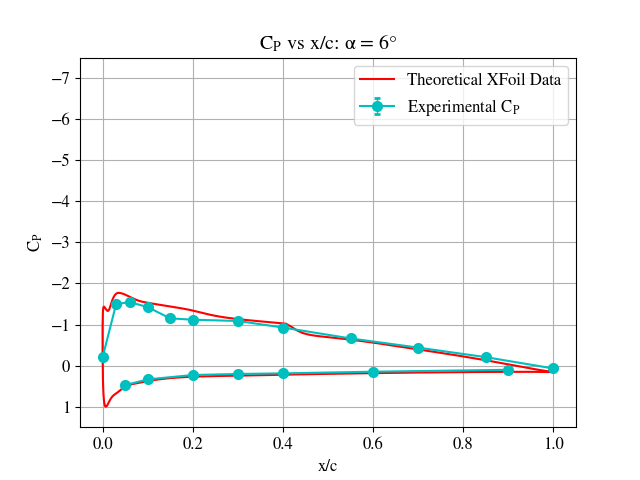
\includegraphics[width=1\textwidth]{Figures/C_p-a6.png}
    \caption{Coefficient of pressure over chord for an alpha of 6\degree.}
    \label{fig:C_p-a6}
  \end{subfigure}
\caption{}
  \label{fig:two1}
\end{figure}

\begin{figure}[h]
  \begin{subfigure}{0.5\textwidth}
    \centering
    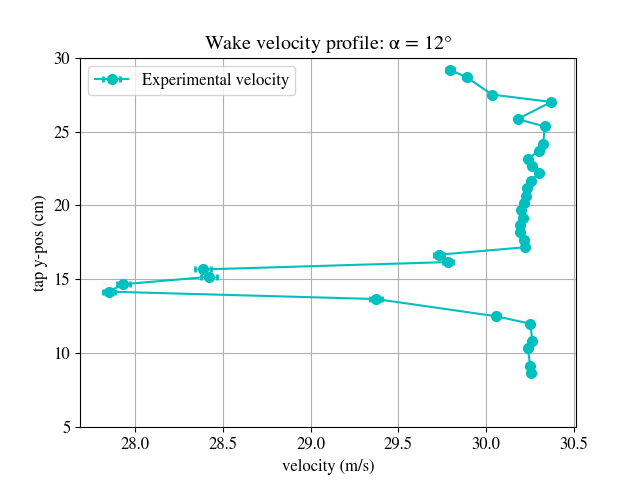
\includegraphics[width=1\linewidth]{Figures/vel-graphs/vel-a12.png}
    \caption{Velocity profile for an alpha of 12\degree.}
    \label{fig:vel-a12}
  \end{subfigure}%
  \begin{subfigure}{0.5\textwidth}
    \centering
    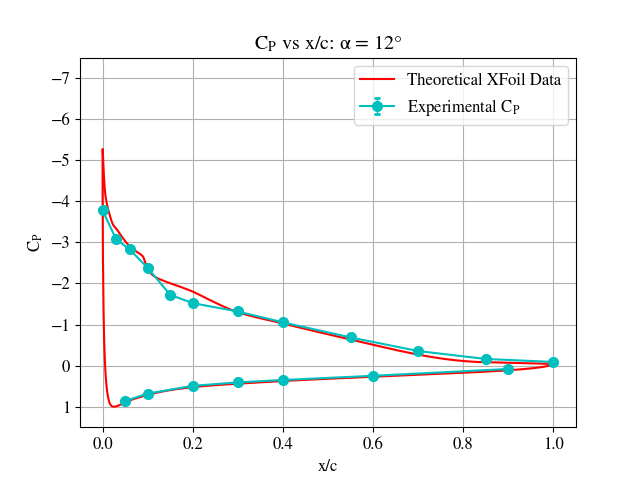
\includegraphics[width=1\textwidth]{Figures/C_p-a12.png}
    \caption{Coefficient of pressure over chord for an alpha of 12\degree.}
    \label{fig:C_p-a12}
  \end{subfigure}
\caption{}
  \label{fig:two2}
\end{figure}

\begin{figure}[h]
  \begin{subfigure}{0.5\textwidth}
    \centering
    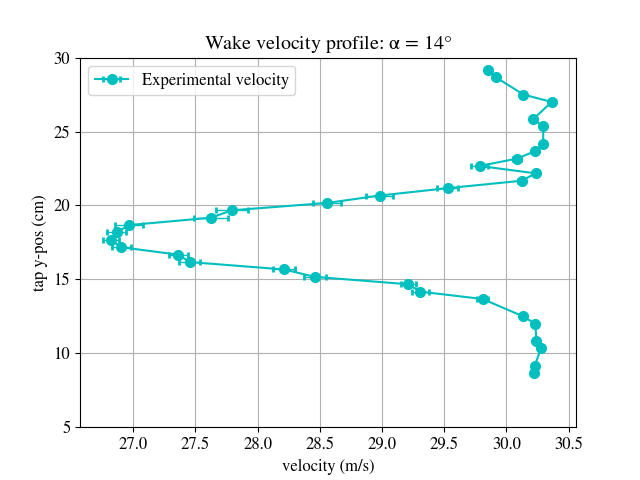
\includegraphics[width=1\linewidth]{Figures/vel-graphs/vel-a14.png}
    \caption{Velocity profile for an alpha of 14\degree.}
    \label{fig:vel-a14}
  \end{subfigure}%
  \begin{subfigure}{0.5\textwidth}
    \centering
    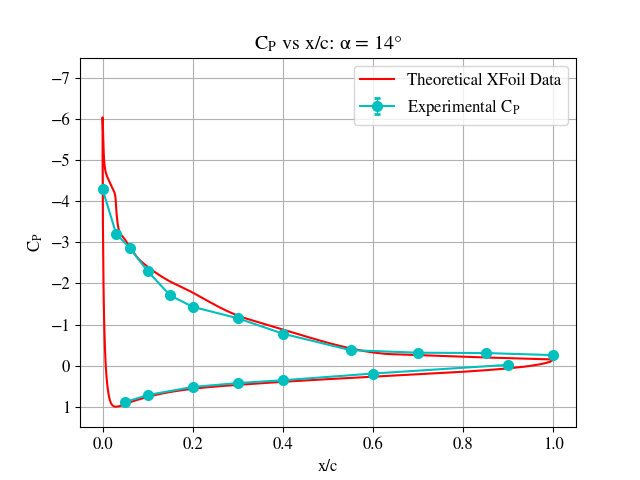
\includegraphics[width=1\textwidth]{Figures/C_p-a14.png}
    \caption{Coefficient of pressure over chord for an alpha of 14\degree.}
    \label{fig:C_p-a14}
  \end{subfigure}
\caption{}
  \label{fig:two3}
\end{figure}

\begin{figure}[h]
  \begin{subfigure}{0.5\textwidth}
    \centering
    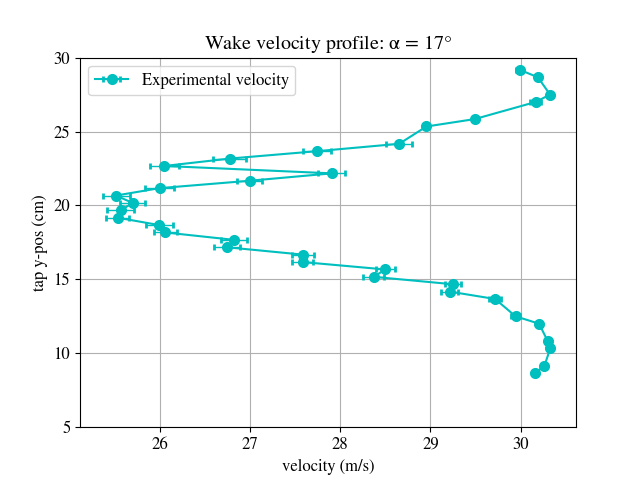
\includegraphics[width=1\linewidth]{Figures/vel-graphs/vel-a17.png}
    \caption{Velocity profile for an alpha of 17\degree.}
    \label{fig:vel-a17}
  \end{subfigure}%
  \begin{subfigure}{0.5\textwidth}
    \centering
    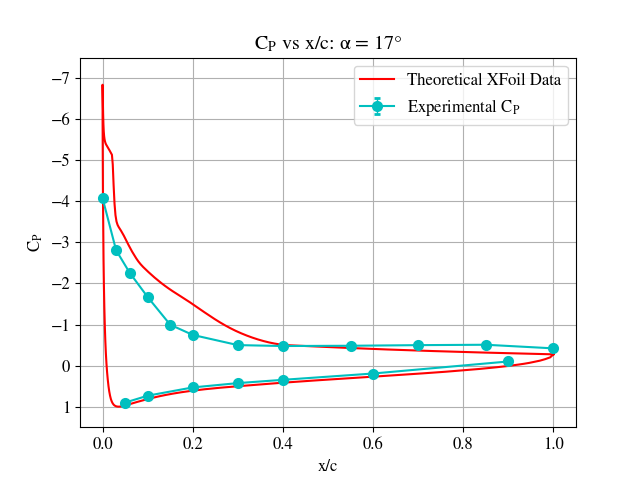
\includegraphics[width=1\textwidth]{Figures/C_p-a17.png}
    \caption{Coefficient of pressure over chord for an alpha of 17\degree.}
    \label{fig:C_p-a17}
  \end{subfigure}
  \caption{}
  \label{fig:two4}
\end{figure}

Perhaps the most noticeable attribute of the pressure distribution graphs is that the pressure over the top of the airfoil is consistently lower than that below it. This confirms the generation of positive lift. However, increasing the angle of attack does not maintain a similar pressure distribution. One observes a shift in the center of pressure towards the leading edge of the airfoil, accompanied by a decrease in the minimum pressure over the airfoil (seen as a peak in the graphs). 

This suggests that the lift close to the leading edge is rapidly increasing but decreasing in other regions. In fact, this trend continues until one can start to see the formation of a plateau in the pressure distribution over the airfoil around an angle of attack of 14°. This points to the separation of flow from the surface of the airfoil. The turbulent flow of air in this region disturbs the smooth pressure gradient and causes a sudden drop in lifting forces. This phenomenon is reconfirmed by observing that the minimum measured pressure coefficient stops decreasing after the critical stall angle. 

When compared to the theoretical XFOIL data, there is a high degree of agreeance between them. Although the theoretical data rarely falls within the plotted uncertainty errorbars, this is likely due to the high degree of error that is difficult to quantify and account for in the measurements. Despite this, the data continuously follows the predicted trends without much deviation and is also able to demonstrate the minimum pressure coefficient peaks with considerable accuracy. However, this does not hold for the higher angles of attack after stall since the predicted minimum continues decreasing but the measurements stagnate. This is likely due to the idealizations and assumptions of the XFOIL software. Since XFOIL implements the panel method of simulating using vortex sheets, it assumes tangential flow and is best suited for attached flow scenarios. It is unable to confidently recognize the stall conditions. 

Another way of observing and confirming the occurrence of stall is by analyzing the wake produced by the airfoil. Placing an array of pressure taps allows us to measure pressure values and thereby approximate a Velocity field in this wake region. We measure an average freestream velocity of 30.31±0.01 m/s and see that for most low angles of attack, the drag (lower-velocity region) is restricted to a small region of the cross-sectional area. However, closer to the stall angle, this region becomes larger due to an increase in turbulent flow. At high angles like 17°, the region of low velocity is rather large and apparently inconsistent (spikes). However, such 'spikes' may also have been the result of mismeasurement of the two rakes' realtive positions and errors therefore. 

\subsection{Comparing the Angle of Attack to the Coefficients of Lift, Drag, and Moment}

\begin{figure}[h]
        \centering        
        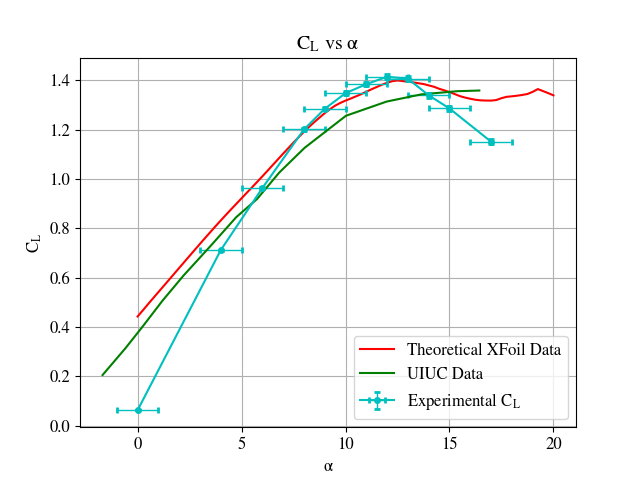
\includegraphics[width=0.5\textwidth]{Figures/C_l-a.png}
        \caption{Coefficient of Lift vs. Angle of Attack.}
        \label{fig:1_C_l-a}
\end{figure}

In Figure \ref{fig:1_C_l-a}, it can be seen that the lift slope of the experimental data represents a considerable concurrence with the patterns of the UIUC and especially XFOIL theoretical data. All three sets of data seem to level off at a similar angle of attack confirming our prediction and measurement for the critical angle of stall. Visibly, the XFOIL prediction doesn't have a drastic downtrend like the experimental data which can likely be attributed to unaccounted 3D effects and the fact the panel method of XFOIL fails to capture flow separation adequately. It is also note-worthy that the experimental $C_L$ lift slope is greater than the predicted values. A possible explanation for such a phenomenon is discrepancies in the airfoil model's aspect ratio used (causing steeper slope) or potential errors in the measured angle of attack which would result in lower lift coefficients being observed. This would be an interesting characteristic to further explore by repeated experiments. 

\begin{figure}[h]
        \centering        
        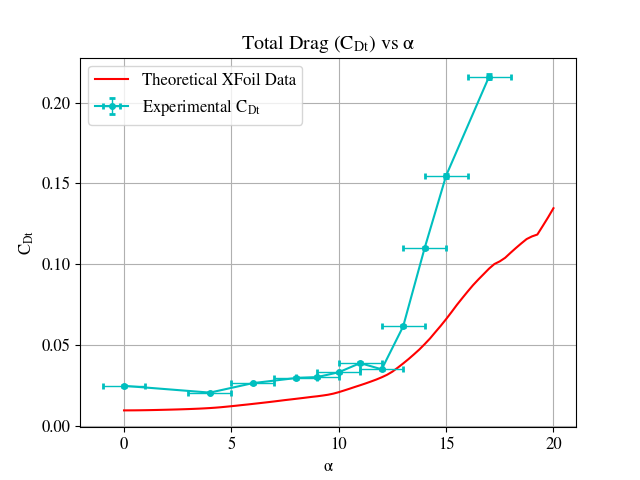
\includegraphics[width=0.5\textwidth]{Figures/C_Dt-a.png}
        \caption{Coefficient of Drag vs. Angle of Attack.}
        \label{fig:1_C_dt-a}
\end{figure}

As seen in Figure \ref{fig:1_C_d-a}, the coefficient of total drag experimental data agrees with the UIUC and XFOIL data trends. The variation from the XFOIL data is considerable but represents the pattern well. However, specifically at high angles of attack, the deviation increases and the drag slope increases drastically close to the stall angle. This profile and inconsistency with data from theoretical sources is expected due to the flow separation from the airfoil and XFOIL's inability to thoroughly model separated flow turbulence.  

\begin{figure}[h]
        \centering        
        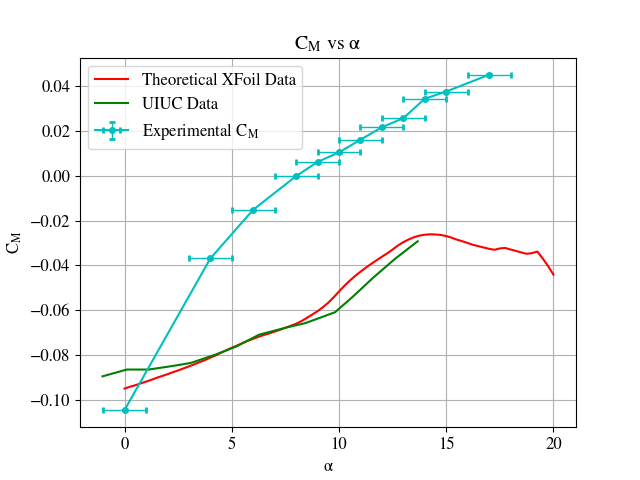
\includegraphics[width=0.5\textwidth]{Figures/C_m-a.png}
        \caption{Coefficient of Moment vs. Angle of Attack.}
        \label{fig:1_C_m-a}
\end{figure}

In Figure \ref{fig:1_C_m-a}, it can be seen that the experimental data for the coefficient of moment varies significantly from both the UIUC and XFOIL data. Even post-stall, the experimental values don't drop as seen by the XFOIL data. The very large difference here is likely attributed to the fact the measurements taken do not particularly include skin friction effects on the airfoil as a result of the limitations of the measurement equipment used. 

It is also important to note that the moment in the airfoil becomes positive as the angle of attack continues to increase. This is rather averse to the theoretical predictions and seems to suggest a 'nose-up moment'. This would lock the airfoil in a positive feedback loop to continue stalling. This does not occur in reality as it is expected that the moment would remain negative and reduce more after stall. The discrepancies in this data don't seem to explained by theory and would warrant further exploration into the experiment.

\begin{figure}[h]
        \centering        
        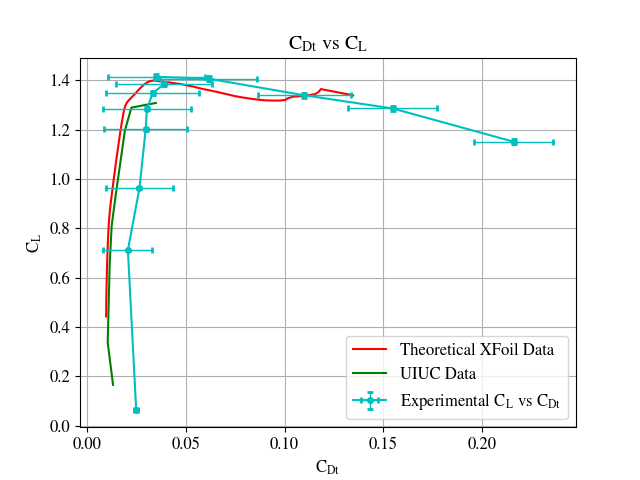
\includegraphics[width=0.5\textwidth]{Figures/C_l-C_d.png}
        \caption{Coefficient of Lift vs. Coefficient of Drag.}
        \label{fig:1_C_l-C_d}
\end{figure}

There is an extensive degree of concurrence between the theoretical and experimental data for \ref{fig:1_C_l-C_d} as it also depicts that theoretical values fall within the uncertainty ranges of the experiment. 
\subsection{Comparison of Pressure Drag and Total Drag}

Pressure drag refers to the drag forces acting on an airfoil directly due to the pressure distribution over its surface. However, total drag is more holistic as it accounts for the drag due to counteracting stress forces of the viscous fluid flow. For the purpose of this lab, those forces were approximated by analyzing the pressure distribution profile in the wake of the airfoil by using data from the rake and comparing it to the experimental freestream velocity. Loss in momentum of the fluid would directly represent the drag enforced upon the airfoil. From Figures \ref{fig:1_C_d-a} and \ref{fig:1_C_Dt-a}, differences between the coefficients of drag and total drag versus angle of attack can be seen. Note that neither graph indicates experimental agreement with the theory. 

It is expected that total drag would be greater than pressure drag, as total drag includes pressure drag as well as skin friction drag (and thus a similar relation would hold between their respective coefficients). In this case, it should be noted that there was a sharp increase in $C_{Dt}$ at around $\alpha = 12\degree$, possibly due to increased cross-sectional area obstructing the flow and increased boundary layer thickness which develops prior to a stall and due to turbulent flow. 

Meanwhile, the $C_D$ Pressure graph does not agree with the proposed theory at all and presents a rapid increase in value quite contrary to that observed in the total pressure plot. In fact, barring the first measurement, the Pressure drag is consistently much higher than the total drag. It is unclear what might have caused such behavior but it could possibly be attributed to discrepancies due to the apparatus. It would be a very important phenomenon to explore in additional controlled experiments or by comparing it to other trials of this lab.  

\begin{figure}[!ht]
        \centering        
        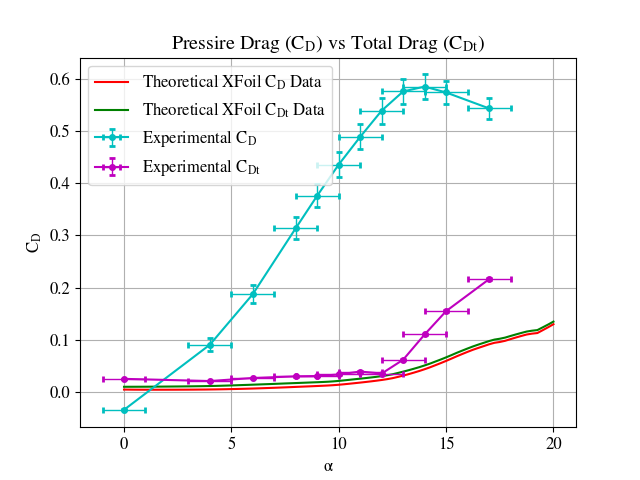
\includegraphics[width=0.5\textwidth]{Figures/C_d-C_dt.png}
        \caption{Coefficient of Total Drag vs. Angle of Attack.}
        \label{fig:1_C_Dt-Cd}
\end{figure}

\section{Uncertainty Analysis and Sources of Error}

\subsection{Quantitative Uncertainties}

Various quantifiable uncertainties that are propagated throughout the analysis are presented in Appendix A. The measurement of the angle of attack can be measured up to $\pm 0.5 \degree$ on the protractor used, which is the bias error. The measurement of the vertical position of the rake can be up to $\pm 1 mm$, the bias error. On the 36 pressure measurements the bias error is assumed to be zero. The precision is of the pressure measurements is calculated by finding the standard deviation across a sample size of a around 90000 points per transducer. Additionally, the integral time constant was found using the \lstinline{statsmodels.api.tsa.acf} function to find $B_{xx}$ and then integrating as follows: 
\begin{equation}\label{eq:autocorrelation}
    T = \int_{0}^{\infty} \frac{\overline{(x(t)-\bar{x})\cdot(x(t-\tau)-\bar{x})}}{\overline{(x(t) - \bar{x})^2}} d\tau = \int_{0}^{\infty} B_{xx} d\tau
\end{equation}
Where $T$ is the integral time constant. The integral time constant was then used to find the number of independent samples which is given by:
\begin{equation}
    N_i = \frac{N}{2T}\frac{1}{f} 
\end{equation}
where $N_i$ is the number of independent samples, $N$ is the total number of samples, and $f$ is the sample frequency which in this experiment was 30kHz. Finally, the $95\%$ confidence interval (the precision uncertainty of the measurement) for pressure measurements was found using the following formula:
\begin{equation}
    P = 1.96*\frac{\sigma}{\sqrt{N_i}}
\end{equation}

\subsection{Qualitative Uncertainties}

A number of possible uncertainties are visible in this experiment that likely have affected the data but cannot be meaningfully quantified. Firstly, the airfoil itself. The pressure taps on the Clark Y airfoil were arranged in line with each other with respect to the incoming airflow. With this setup an up-stream tap's effect on the airflow may impact the pressure on the down-stream taps, giving inaccurate measurements not representative of the actual airfoil. With respect to the airflow through the wind tunnel, not much information is known about the consistency and stability of the flow. The flow is very likely not completely linear and the speed may fluctuate with time and the frequency of the pump system may align with measurement frequencies, adding uncertainties to the measurements. Additionally, the pressure transducer (Scanivalve CTLR10 P/S2-S6) is quite an old product with little information known about its errors and tolerances. In addition to errors in measurement present at manufacturing, over its significant life these error have likely increased due to aging components. It was also discovered that one or more of the pressure taps were giving erratic values likely a result of clogging or damage to the pressure tubes. Lastly, the distance of the trailing edge of the airfoil to the rake was larger than would be optimal. The large distance may present loses in resolution and increased turbulence.

\section{Conclusion}

This experiment investigated the pressure distribution and nondimensional coefficients of flow around a Clark Y airfoil, using a Scanivalve pressure transducer system. In addition, a rake of pressure taps was utilized to characterize the wake caused downstream of the airfoil. Data was collected at several different positive angles of attack ranging from 0° to 17°. The results were subsequently analyzed to identify the critical stall angle and study the effects such stall would have on various properties and force coefficient distributions around the airfoil. The results were compared with simulations from XFOIL and existing literature, giving a stall angle of $\alpha \approx 14 \deg$.The dimensionless coefficients demonstrated visible trends: 

Although the data for pressure distribution was relatively consistent with simulated numbers, inconsistencies could be attributed to the mathematical model used by XFOIL. Since it uses a panel approach, it was insufficient in predicting the detached flow and was less accurate at higher angles of attack following stall. Further sources of error due to the short-falls of the setup itself likely resulted in bias in the measurements. For the coefficient of lift and total drag, the trend of the experimental data generally matched that of other sources though the magnitude and slopes varied. However, post-stall characteristics and the magnitude of the values and their slopes vary significantly. The exaggerated measurements in the moment coefficient do not agree with the values for the corresponding theory. This could potentially be explained by the contribution of turbulent flow and by factors not included in the theoretical simulations, akin to skin friction or inconsistencies in test apparatus. 

In the future, it would be beneficial to explore a more consistent, repeatable, and reliable experimentation method for collecting experimental data. Difficulties in ensuring accurate angles of attack and rake positions likely contributed to larger discrepancies. Furthermore, researching alternative sources of theoretical data would be beneficial if it would be possible to predict flow separation and stall more accurately. An increase in the number of pressure taps and staggering them relative to each other over the airfoil would also allow for a more refined and less noisy collection of pressure data over the airfoil surface. Future iterations should focus on higher angle resolution to reduce stall uncertainty, with cleaning of pressure taps, re-calibration or replacement of the protractor for precise angle measurements, and exploring alternative moment measurement devices to account for skin friction effects. It would also be very interesting to explore the specific source of error resulting in the discrepancies in Pressure Drag and Moment data.

% This comprehensive investigation showed the successful characterization of the Clark Y airfoil while emphasizing avenues for refinement in future experiments.

\newpage
\bibliographystyle{ieeetr} % We choose the "plain" reference style
\bibliography{cite}


\newpage
% \appendix

\begin{appendices}

\section{Uncertainty Propagation Formulas}

\subsection{Lift, Drag, Moment, and Pressure Coefficients}

These are the equations used for the relevant dimensionless coefficients:

\begin{equation}
    \delta C_L = \sqrt{(\tfrac{\delta L}{q_\infty c} )^2 + (\tfrac{L}{q_\infty ^2 c} + \delta q_\infty)^2}
\end{equation}

\begin{equation}
    \delta C_D_p = \sqrt{(\tfrac{\delta D_p}{q_\infty c} )^2 + (\tfrac{D_p}{q_\infty ^2 c} + \delta q_\infty)^2}
\end{equation}

\begin{equation}
    \delta C_D_t &= \sqrt{(\tfrac{\delta D_t}{q_\infty c} )^2 + (\tfrac{D_t}{q_\infty ^2 c} + \delta q_\infty)^2}
\end{equation}

\begin{equation}
    \delta C_M &= \sqrt{(\tfrac{\delta M}{q_\infty c} )^2 + (\tfrac{M}{q_\infty ^2 c} + \delta q_\infty)^2}
\end{equation}

\begin{equation}
    \delta C_p &= \sqrt{(\tfrac{\delta (P_s-P_\infty)}{q_\infty} )^2 + (\tfrac{(P_s-P_\infty)\times \delta q_\infty}{q_\infty ^2})^2}
\end{equation}

\subsection{Lift, and Pressure, and Total Drag}

The lift, pressure drag, and total drag along the airfoil were calculated using the error equations below:

\begin{equation}
    \delta D_t &= \sqrt{\sum_{i=0}^N [(\tfrac{\partial D_t}{\partial v_i} \delta v_i)^2 + (\tfrac{\partial D_t}{\partial v_{i + 1}} \delta v_{i + 1})^2 + (\tfrac{\partial D_t}{\partial U_\infty} \delta U_\infty)^2]} 
\end{equation}

\begin{equation}
    \delta L &= \sqrt{(\cos(\alpha) \delta N)^2 + (\sin(\alpha) \delta A)^2 + ((-N\sin(\alpha) - A \cos(\alpha)) \delta \alpha)^2}
\end{equation}

\begin{equation}
    \delta D_p &= \sqrt{(\sin(\alpha) \delta N)^2 + (\cos(\alpha) \delta A)^2 + ((-N\cos(\alpha) - A \sin(\alpha)) \delta \alpha)^2}
\end{equation}

\subsection{Pressure}

Pressure measurements were taken for 3 seconds at a sampling rate of 30000 Hz and a time average was taken. The precision error of the measurements was found with a confidence interval of 95\% as follows:

\begin{equation}
    \delta (P_S - P_\infty) &= \delta (P_T - P_\infty) &= 1.96 \tfrac{\sigma}{\sqrt{N}}
\end{equation}

where $N &= \frac{t_s}{2 \tau}$

\subsection{Angle Of Attack}

The uncertainty of the angle of attack based on the measurement technique used (protractor) is:

\begin{equation}
    \delta \alpha &= 1 \deg
\end{equation}

\subsection{Freestream Flow and Wake Velocity}

The freestream velocity was calculated using an average of the top and bottom wake velocities using the error propogation below:

\begin{equation}
    \delta U_\infty &= \sqrt{(\tfrac{1}{2} \delta v_{top})^2 + (\tfrac{1}{2} \delta v_{bottom})^2}
\end{equation}

\begin{equation}
    \delta v &= \frac{\delta(P_t - P_\infty)}{\sqrt{2\rho(P_t - P_\infty)}}
\end{equation}

\subsection{Freestream Dynamic Pressure}

The freestream dynamic Uncertainty was calculated using the equation below where density is considered constant due to the low speeds of the tunnel:

\begin{equation}
    q_\infty &= \tfrac{1}{2} \rho U_\infty^2
\end{equation}

\begin{equation}
    \delta q_\infty &= \rho U_\infty \times \delta U_\infty
\end{equation}

\subsection{Normal and Axial Force}

The normal and axial forces along the airfoil were calculated by integrating the pressure distribution measured and error propogated with the following formulas:

\begin{equation}
    \delta N = \sqrt{\sum_{i=0}^N [(\tfrac{\partial N}{\partial p_{u,i}} \delta p_{u,i})^2 + (\tfrac{\partial N}{\partial p_{u,i+1}} \delta p_{u,i+1})^2 + (\tfrac{\partial N}{\partial p_{l,i}} \delta p_{l,i})^2 + (\tfrac{\partial N}{\partial p_{l,i+1}} \delta p_{l,i+1})^2]}
\end{equation}

\begin{equation}
    \delta A = \sqrt{\sum_{i=0}^N [(\tfrac{\partial A}{\partial p_{u,i}} \delta p_{u,i})^2 + (\tfrac{\partial A}{\partial p_{u,i+1}} \delta p_{u,i+1})^2 + (\tfrac{\partial A}{\partial p_{l,i}} \delta p_{l,i})^2 + (\tfrac{\partial A}{\partial p_{l,i+1}} \delta p_{l,i+1})^2]}
\end{equation}
where using the trapezoidal integration rule we use the substitutions:
\begin{align*}
    \tfrac{\partial N}{\partial p_{u,i}} &= -\tfrac{1}{2} (x_{u,i+1} - x_{u,i}) \times cos(\theta_{u,i}) \times \Delta S \\
    \tfrac{\partial N}{\partial p_{u,i+1}} &= -\tfrac{1}{2} (x_{u,i+1} - x_{u,i}) \times cos(\theta_{u,i+1}) \times \Delta S \\
    \tfrac{\partial N}{\partial p_{l,i}} &= -\tfrac{1}{2} (x_{l,i+1} - x_{l,i}) \times cos(\theta_{l,i}) \times \Delta S\\
    \tfrac{\partial N}{\partial p_{l,i+1}} &= -\tfrac{1}{2} (x_{l,i+1} - x_{l,i}) \times cos(\theta_{l,i+1}) \times \Delta S\\
    \tfrac{\partial A}{\partial p_{u,i}} &= -\tfrac{1}{2} (x_{u,i+1} - x_{u,i}) \times sin(\theta_{u,i}) \times \Delta S\\
    \tfrac{\partial A}{\partial p_{u,i+1}} &= -\tfrac{1}{2} (x_{u,i+1} - x_{u,i}) \times sin(\theta_{u,i+1}) \times \Delta S\\
    \tfrac{\partial A}{\partial p_{l,i}} &= -\tfrac{1}{2} (x_{l,i+1} - x_{l,i}) \times sin(\theta_{l,i}) \times \Delta S\\
    \tfrac{\partial A}{\partial p_{l,i+1}} &= -\tfrac{1}{2} (x_{l,i+1} - x_{l,i}) \times sin(\theta_{l,i+1}) \times \Delta S
\end{align*}

\subsection{Leading Edge Moment}

As with normal and axial force, the moment was calculated by integrating the pressure distribution and using the follow error formulas:

\begin{equation}
    \delta M_{LE} &= \sqrt{\sum_{i=0}^N [(\tfrac{\partial M_{LE}}{\partial p_{u,i}} \times \delta p_{u,i})^2 + (\tfrac{\partial M_{LE}}{\partial p_{u,i+1}} \times \delta p_{u,i+1})^2 + (\tfrac{\partial M_{LE}}{\partial p_{l,i}} \times \delta p_{l,i})^2 + (\tfrac{\partial M_{LE}}{\partial p_{l,i+1}} \times \delta p_{l,i+1})^2]}
\end{equation}
where using the trapezoidal integration rule we use the substitutions:
\begin{align*}
    \tfrac{\partial M_{LE}}{\partial p_{u,i}} &= \tfrac{1}{2} (x_{u,i+1} - x_{u,i}) \times (x_{u,i} cos(\theta_{u,i}) - y_{u,i} sin(\theta_{u,i})) \times \Delta S \\
    \tfrac{\partial M_{LE}}{\partial p_{u,i+1}} &= \tfrac{1}{2} (x_{u,i+1} - x_{u,i}) \times (x_{u,i+1} cos(\theta_{u,i+1}) - y_{u,i+1} sin(\theta_{u,i+1})) \times \Delta S \\
    \tfrac{\partial M_{LE}}{\partial p_{l,i}} &= \tfrac{1}{2} (x_{l,i+1} - x_{l,i}) \times (- x_{l,i} cos(\theta_{l,i}) + y_{l,i} sin(\theta_{u,i})) \times \Delta S \\
    \tfrac{\partial M_{LE}}{\partial p_{l,i+1}} &= \tfrac{1}{2} (x_{l,i+1} - x_{l,i}) \times (- x_{l,i+1} cos(\theta_{l,i+1}) + y_{l,i+1} sin(\theta_{l,i+1})) \times \Delta S\\
\end{align*}

\newpage
\section{Code}
All code utilized for this lab can be found at the following Github repository: \url{https://github.com/Gigigo16/AER303-Airfoil}
\subsection{filter.m}
\begin{minted}{matlab}
clear 
nums = [0,4,6,8,9,10,11,12,13,14,15,17];
for j = 1:length(nums)
    clear data
    data = load(".\data\Unfiltered\Experimental_data_"+nums(j)+".mat");
    data.wpdata2;
    spdatafilt = zeros(19, 90090);
    wpdatafilt = zeros(19, 90090);
    wpdata2filt = zeros(19, 90090);
    for i = 1:19
        spdatafilt(i, :) = SigFilt(data.spdata(i, :));
        if i<18
            wpdatafilt(i, :) = SigFilt(data.wpdata(i, :));
            wpdata2filt(i, :) = SigFilt(data.wpdata2(i, :));
        end
    end
    data.spdata = spdatafilt;
    data.wpdata = wpdatafilt;
    data.wpdata2 = wpdata2filt;
    data.wpdata2;
    save(".\data\Filtered\Experimental_data_"+nums(j)+".mat","-struct","data")
end
%%
function [Sig_filt] = SigFilt(Sig)

[zF1, pF1, kF1]         = cheby2(4, 20, (30 / (30000 / 2)), 'low');
[bF1, aF1]              = zp2tf(zF1, pF1, kF1);
Sig_filt                = filtfilt(bF1, aF1, Sig);

end
\end{minted}
\subsection{Main.py}
\begin{minted}{python}
"""
Main script for running all data processing and plotting.
    {Depenancies}: scipy, matplotlib, numpy
"""
# IMPORTS
#####################
# Dependancies
from scipy import io
import matplotlib.pyplot as plt
import numpy as np
import csv

# Custom Functions/libraies
from ReynoldsNumber import *
from Forces import *
from Velocity import *
from Coefficients import *
from PressuretoCSV import *
from Uncertainty import *
from Graphing import *


# DEFINITIONS
########################
# airfoil tap positions: 
air_top_tap_pos = [0, 0.03, 0.06, 0.10, 0.15, 0.20, 0.30, 0.40, 0.55, 0.70, 0.85, 1.00]
air_bot_tap_pos = [0.90, 0.60, 0.40, 0.30, 0.20, 0.10, 0.05]

# airfoil cord length
c = 0.1 #m

# Angles of Attack
alpha = [0, 4, 6, 8, 9, 10, 11, 12, 13, 14, 15, 17] #12
dalpha = 1 #deg uncertainty in AoA

# calibration data
gain = 115 # From in lab calibration code
offset = 50 # From in lab calibration code
Hg2Pa = 9.80665 #inHg to Pa convertion factor

# baselines of rake positions:
y_0 = np.array([12, 12, 11.5, 11, 11.5, 11, 11.5, 12.5, 11.5, 12, 12.4, 12]) - 3.33 # inital position of the bottom port
dir = [1, -1, -1, 1, -1, 1, 1, -1, -2, 1, -1, 1] #direction rake was moved -1 = down 1 = up

print("Loading Clark Y Airfoil Coordinates...")
# LOADING CLARK_Y_AIRFOIL COORDINATES
##############################
with open(".\data\Clark_Y_Airfoil.csv", newline='') as f:
    points = csv.reader(f, delimiter=';')
    data = list(points)
    data.pop(0)

# Converting to float
i = 0
for row in data:
    data[i] = list(map(float, row)) 
    i += 1

is_top = True
airfoil_top = []
airfoil_bot = []
for i in range(0,len(data)):
    if i != 0 and float(data[i][0]) == float(0.0):
        is_top = False
    if is_top and float(data[i][0]) in air_top_tap_pos:
        airfoil_top.append([float(data[i][0]), float(data[i][1])])
    elif not is_top and float(data[i][0]) in air_bot_tap_pos:
        airfoil_bot.append([float(data[i][0]), float(data[i][1])])


# Convert to np.array
airfoil_top = np.array(airfoil_top)*0.1  # Multiplying values by cord length (values given are per unit cord)
airfoil_bot = np.array(airfoil_bot)*0.1 # Multiplying values by cord length (values given are per unit cord)

print("Loading Experimental Data...")

# Data array initialization
pressure_data = []
rake_press = []
rake_press_err = []
y_rake_pos = []
Cl_list = []
dCl_list = []
Cd_list = []
dCd_list = []
Cm_list = []
dCm_list = []
Cdt_list = []
dCdt_list = []

# PROCESSING DATA
########################
print("=========================================")
print("Beginning Analysis...")
print("=========================================")
for i,a in enumerate(alpha):
    print("Processing AoA = %d..."%a)

    # this data was pre-filtered in matlab
    # errors were calculated in errcalc.py
    data_raw = io.loadmat(".\data\Filtered\Experimental_data_%d.mat"%a)
    # ['__header__', '__version__', '__globals__', 'AoA', 'ask', 'None', 
    # 'f_s', 'i', 'k', 'p_airfoil', 'p_rake1', 'p_rake2', 'prompt', 'spdata', 'sptime', 
    # 't_s', 'wpdata', 'wpdata2', 'wptime1', 'wptime2', 'x', 'y', 'y2', '__function_workspace__']

    # data calibration:
    p_top = (data_raw['p_airfoil'][0][0:12]*gain + offset)*Hg2Pa
    p_bot = (data_raw['p_airfoil'][0][12:19]*gain + offset)*Hg2Pa
    p_r1 = (data_raw['p_rake1']*gain + offset)*Hg2Pa
    p_r2 = (data_raw['p_rake2']*gain + offset)*Hg2Pa
    
    p = (data_raw['p_airfoil'][0]*gain + offset)*Hg2Pa
    pressure_data.append(list(map(float, p)))
    
    # Initializing error arrays
    p_r1_err = np.zeros_like(p_r1) #temp
    p_r2_err = np.zeros_like(p_r2) #temp
    p_top_err = np.zeros_like(p_top) #temp
    p_bot_err = np.zeros_like(p_bot) #temp
    
    # Parsing error data from CSV files
    with open('data\CSV\dP_airfoil.csv') as f:
        reader = csv.reader(f)
        data_err_a = list(reader)
        data_err_a = [eval(e) for e in data_err_a[i]]
        p_top_err = data_err_a[0:12]
        p_bot_err = data_err_a[12:19]
    with open('data\CSV\dP_rakepos1.csv') as f:
        reader = csv.reader(f)
        data_err_r1 = list(map(np.float64,reader))
        p_r1_err = np.array(data_err_r1)[i]

    with open('data\CSV\dP_rakepos2.csv') as f:
        reader = csv.reader(f)
        data_err_r2 = list(map(np.float64,reader))
        p_r2_err = np.array(data_err_r2)[i]

    
    # finding the wake velocity distribution:
    pos_r1 = y_0[i]
    pos_r2 = y_0[i] + dir[i]*0.5
    
    U_inf, U_inf_err, V_r, V_r_err, V_pos, P_comb, P_comb_err = Velocity(p_r1, p_r2, p_r1_err, p_r2_err, pos_r1, pos_r2)

    rake_press.append(list(map(float, P_comb)))
    rake_press_err.append(list(map(float, P_comb_err)))
    y_rake_pos.append(list(map(float, V_pos)))

    # Plotting velocity distribution
    VelGraph(a, V_r, V_r_err, V_pos)


    #finding the dynamic freestream pressure
    q_inf, q_inf_err = DynPressure(U_inf, U_inf_err)



    #finding the lift and total drag
    Dt, Dt_err = TotalDrag(V_pos/100, V_r, V_r_err, U_inf, U_inf_err)

    # Finding normal, axial forces and moment forces
    N, dN = NormalForce(p_top, p_bot, p_top_err, p_bot_err, airfoil_top, airfoil_bot, a)
    A, dA = AxialForce(p_top, p_bot, p_top_err, p_bot_err, airfoil_top, airfoil_bot, a)
    M, dM = MomentLE(p_top, p_bot, p_top_err, p_bot_err, airfoil_top, airfoil_bot, a)

    # Finding lift and drag forces
    L, dL = LiftForce(a, dalpha, N, dN, A, dA)
    D, dD = PressureDragForce(a, dalpha, N, dN, A, dA)

    # Finding pressure coefficients
    Cp_top, Cp_bot, Cp_top_err, Cp_bot_err = Cpressure(p_top, p_bot, p_top_err, p_bot_err, q_inf, q_inf_err)

    # total drag coefficient
    Cdt, dCdt = Ctotaldrag(Dt, Dt_err, q_inf, q_inf_err, c)

    # finding remaining Coefficients
    Cl, dCl, Cd, dCd, Cm, dCm =Coefficients(L, dL, D, dD, M, dM, q_inf, q_inf_err, c)

    # Plotting Cp distribution
    CpGraph(a, Cp_top, Cp_bot, Cp_top_err, Cp_bot_err)

    # Storing data
    Cl_list.append(Cl)
    Cd_list.append(Cd)
    Cm_list.append(Cm)
    Cdt_list.append(Cdt)
    dCl_list.append(dCl)
    dCd_list.append(dCd)
    dCm_list.append(dCm)
    dCdt_list.append(dCdt)



print("Analysis Complete...")
print("=========================================")
# Plotting data
CoeffGraph(alpha, Cl_list, dCl_list, Cd_list, dCd_list, Cm_list, dCm_list, Cdt_list, dCdt_list)

print("Saving Data CSVs...")
# Saving data raw data to CSV
PressuretoCSV(alpha, np.array(pressure_data))
RakePressuretoCSV(alpha, np.array(rake_press), np.array(y_rake_pos))
RakeUncertaintytoCSV(alpha, np.array(rake_press_err), np.array(y_rake_pos))
\end{minted}

\subsection{errorcalcs.py}
\begin{minted}{python}
"""
Script for calculating all measured data uncertainties at all AoAs and ports.
    {Depenancies}: scipy, matplotlib, numpy
"""
# IMPORTS
#####################
# Dependancies
from scipy import io
import matplotlib.pyplot as plt
import numpy as np
import csv

# Custom Functions/libraies
from Uncertainty import *


# DEFINITIONS
########################
# airfoil tap positions: 
air_top_tap_pos = [0, 0.03, 0.06, 0.10, 0.15, 0.20, 0.30, 0.40, 0.55, 0.70, 0.85, 1.00]
air_bot_tap_pos = [0.90, 0.60, 0.40, 0.30, 0.20, 0.10, 0.05]
gain = 115 # From in lab calibration code
offset = 50 # From in lab calibration code
Hg2Pa = 9.80665 #inHg to Pa convertion factor

# Angles of Attack
alpha = [0, 4, 6, 8, 9, 10, 11, 12, 13, 14, 15, 17]

dP_a = np.zeros((len(alpha), 19))
dP_r1 = np.zeros((len(alpha), 17))
dP_r2 = np.zeros((len(alpha), 17))

for i, a in enumerate(alpha):

    data = io.loadmat(".\data\Filtered\Experimental_data_%d.mat"%a)
    # ['__header__', '__version__', '__globals__', 'AoA', 'ask', 'None', 
    # 'f_s', 'i', 'k', 'p_airfoil', 'p_rake1', 'p_rake2', 'prompt', 'spdata', 'sptime', 
    # 't_s', 'wpdata', 'wpdata2', 'wptime1', 'wptime2', 'x', 'y', 'y2', '__function_workspace__']

    #error calcs:
    for k in range(1, 20):
        dP_a[i, k-1] = DataErr((data['spdata'][k-1]*gain + offset)*Hg2Pa)
        # Bxx = DataErr((data['spdata'][0]*gain + offset)*Hg2Pa)
        if (k < 18):
            dP_r1[i, k-1] = DataErr((data['wpdata'][k-1]*gain + offset)*Hg2Pa)
            dP_r2[i, k-1] = DataErr((data['wpdata2'][k-1]*gain + offset)*Hg2Pa)

# Saving data to CSV files

np.savetxt("data\CSV\dP_airfoil.csv", dP_a, delimiter=",")
np.savetxt("data\CSV\dP_rakepos1.csv", dP_r1, delimiter=",")
np.savetxt("data\CSV\dP_rakepos2.csv", dP_r2, delimiter=",")
\end{minted}
\subsection{Forces.py}
\begin{minted}{python}
import numpy as np

def NormalForce(p_top: np.array, p_bot: np.array, p_err_top: np.array, p_err_bot: np.array, top_p_pos: np.array, bot_p_pos: np.array, alpha):
    '''
    Returns the Normal force for pressure distribution.

    Parameters:
    -----------   
    p_top : np.array
        top airfoil pressure distribution
    p_bot : np.array
        bottom airfoil pressure distribution
    p_err_top : np.array
        top airfoil perssure error
    p_err_bot : np.array
        bottom airfoil perssure error
    top_p_pos : list
        top airfoil pressure tap positions [x; y]
    bot_p_pos : list
        bottom airfoil pressure tap positions [x; y]

    Returns:
    --------
    n: Normal Force
    dn: Normal Force uncertainty
    '''
    x_upper = [row[0] for row in top_p_pos]
    x_lower = [row[0] for row in bot_p_pos]
    y_upper = [row[1] for row in top_p_pos]
    y_lower = [row[1] for row in bot_p_pos]

    theta_upper= np.arctan(np.diff(y_upper)/np.diff(x_upper))
    theta_lower= np.arctan(np.diff(y_lower)/np.diff(x_lower))


    ds_upper = np.sqrt(np.diff(x_upper)**2 + np.diff(y_upper)**2)
    ds_lower = np.sqrt(np.diff(x_lower)**2 + np.diff(y_lower)**2)

    x_upper = np.diff(x_upper)
    x_lower = np.diff(x_lower)
    y_upper = np.diff(y_upper)
    y_lower = np.diff(y_lower)
    
    n = 0
    dn = 0
    # Trapezoidal numerical integration
    for i in range(len(ds_upper)):
        n += -0.5 * (p_top[i] + p_top[i+1]) * np.cos(theta_upper[i]) * ds_upper[i]
        dn += (-0.5*p_err_top[i]*np.cos(theta_upper[i])*ds_upper[i])**2 + (-0.5*p_err_top[i+1]*np.cos(theta_upper[i])*ds_upper[i])**2
    
    for i in range(len(ds_lower)):
        n += 0.5 * (p_bot[i] + p_bot[i+1]) * np.cos(theta_lower[i]) * ds_lower[i]
        dn += (0.5*p_err_bot[i]*np.cos(theta_lower[i])*ds_lower[i])**2 + (0.5*p_err_bot[i+1]*np.cos(theta_lower[i])*ds_lower[i])**2
    
    # Calculating error (position error assumed to be 0)
    dn = np.sqrt(dn)
    
    return n, dn

def AxialForce(p_top: np.array, p_bot: np.array, p_err_top: np.array, p_err_bot: np.array, top_p_pos: np.array, bot_p_pos: np.array, alpha):
    '''
    Returns the Axial force for pressure distribution.

    Parameters:
    -----------   
    p_top : np.array
        top airfoil pressure distribution
    p_bot : np.array
        bottom airfoil pressure distribution
    p_err_top : np.array
        top airfoil perssure error
    p_err_bot : np.array
        bottom airfoil perssure error
    top_p_pos : list
        top airfoil pressure tap positions [x; y]
    bot_p_pos : list
        bottom airfoil pressure tap positions [x; y]
    Returns:
    --------
    a: Axial Force
    da: Axial Force uncertainty
    '''
    x_upper = [row[0] for row in top_p_pos]
    x_lower = [row[0] for row in bot_p_pos]
    y_upper = [row[1] for row in top_p_pos]
    y_lower = [row[1] for row in bot_p_pos]
    
    theta_upper= np.arctan(np.diff(y_upper)/np.diff(x_upper))
    theta_lower= np.arctan(np.diff(y_lower)/np.diff(x_lower))
    
    ds_upper = np.sqrt(np.diff(x_upper)**2 + np.diff(y_upper)**2)
    ds_lower = np.sqrt(np.diff(x_lower)**2 + np.diff(y_lower)**2)
    
    x_upper = np.diff(x_upper)
    x_lower = np.diff(x_lower)
    y_upper = np.diff(y_upper)
    y_lower = np.diff(y_lower)

    a = 0
    da = 0

    # Trapezoidal numerical integration
    for i in range(len(ds_upper)):
        a += -0.5 * (p_top[i] + p_top[i+1]) * np.sin(theta_upper[i]) * ds_upper[i]
        da += (-0.5*p_err_top[i]*np.sin(theta_upper[i])*ds_upper[i])**2 + (-0.5*p_err_top[i+1]*np.sin(theta_upper[i])*ds_upper[i])**2
    
    for i in range(len(ds_lower)):
        a += 0.5 * (p_bot[i] + p_bot[i+1]) * np.sin(theta_lower[i]) * ds_lower[i]
        da += (0.5*p_err_bot[i]*np.sin(theta_lower[i])*ds_lower[i])**2 + (0.5*p_err_bot[i+1]*np.sin(theta_lower[i])*ds_lower[i])**2
    
    # Calculating error (position error assumed to be 0)
    da = np.sqrt(da)
    
    return a, da

def LiftForce(alpha: float, dalpha: float, n: float, dn: float, a: float, da: float):
    '''
    Returns the Lift force for given normal and axial forces at given AoA.

    Parameters:
    -----------   
    alpha : float
        angle of attack (degrees)
    dalpha : float
        angle of attack uncertainty (degrees)
    n : float
        Normal force (Newtons)
    dn : float
        Normal force uncertainty (Newtons)
    a : float
        Axial force (Newtons)
    da : float
        Axial force uncertainty (Newtons)
    Returns:
    --------
    l: Lift Force
    dl: Lift Force uncertainty
    '''

    l = n * np.cos(np.deg2rad(alpha)) - a * np.sin(np.deg2rad(alpha))
    dl =  np.sqrt((np.cos(np.deg2rad(alpha)) * dn)**2 + (np.sin(np.deg2rad(alpha)) * da)**2 + ((-n*np.sin(np.deg2rad(alpha)) - a*np.cos(np.deg2rad(alpha)))*np.deg2rad(dalpha))**2)

    return l, dl

def PressureDragForce(alpha: float, dalpha: float, n: float, dn: float, a: float, da: float):
    '''
    Returns the Pressure drag force for given normal and axial forces at given AoA.

    Parameters:
    -----------   
    alpha : float
        angle of attack (degrees)
    dalpha : float
        angle of attack uncertainty (degrees)
    n : float
        Normal force (Newtons)
    dn : float
        Normal force uncertainty (Newtons)
    a : float
        Axial force (Newtons)
    da : float
        Axial force uncertainty (Newtons)
    Returns:
    --------
    dp: Pressure Drag Force
    ddp: Pressure Drag Force uncertainty
    '''

    dp = n * np.sin(np.deg2rad(alpha)) + a * np.cos(np.deg2rad(alpha))
    ddp =  np.sqrt((np.sin(np.deg2rad(alpha)) * dn)**2 + (np.cos(np.deg2rad(alpha)) * da)**2 + ((n*np.cos(np.deg2rad(alpha)) - a*np.sin(np.deg2rad(alpha)))*np.deg2rad(dalpha))**2)

    return dp, ddp

def MomentLE(p_top: np.array, p_bot: np.array, p_err_top: np.array, p_err_bot: np.array, top_p_pos: np.array, bot_p_pos: np.array, alpha):
    '''
    Returns the Moment about the leading edge 
    acting on the airfoil for given pressure distribution.

    Parameters:
    -----------   
    p_top : np.array
        top airfoil pressure distribution
    p_bot : np.array
        bottom airfoil pressure distribution
    p_err_top : np.array
        top airfoil perssure error
    p_err_bot : np.array
        bottom airfoil perssure error
    top_p_pos : list
        top airfoil pressure tap positions [x; y]
    bot_p_pos : list
        bottom airfoil pressure tap positions [x; y]
    Returns:
    --------
    m: Moment 
    dm: Moment uncertainty
    '''
    x_upper = [row[0] for row in top_p_pos]
    x_lower = [row[0] for row in bot_p_pos]
    y_upper = [row[1] for row in top_p_pos]
    y_lower = [row[1] for row in bot_p_pos]
    theta_upper= np.arctan(np.diff(y_upper)/np.diff(x_upper))
    theta_lower= np.arctan(np.diff(y_lower)/np.diff(x_lower))
    
    ds_upper = np.sqrt(np.diff(x_upper)**2 + np.diff(y_upper)**2)
    ds_lower = np.sqrt(np.diff(x_lower)**2 + np.diff(y_lower)**2)   

    x_upper = np.diff(x_upper)
    x_lower = np.diff(x_lower)
    y_upper = np.diff(y_upper)
    y_lower = np.diff(y_lower)

    m = 0
    dm = 0

    for i in range(len(ds_upper)):
        m += 0.5*(p_top[i] + p_top[i+1])*np.cos(theta_upper[i]-np.deg2rad(alpha))*x_upper[i]*ds_upper[i]
        m += -0.5*(p_top[i] + p_top[i+1])*np.sin(theta_upper[i]-np.deg2rad(alpha))*y_upper[i]*ds_upper[i]

        dm += (0.5*np.cos(theta_upper[i])*x_upper[i]*ds_upper[i]-0.5*np.sin(theta_upper[i])*y_upper[i]*ds_upper[i]*p_err_top[i])**2

    for i in range(len(ds_lower)):
        m += 0.5*(p_bot[i] + p_bot[i+1])*np.cos(theta_lower[i]-np.deg2rad(alpha))*x_lower[i]*ds_lower[i]
        m += 0.5*(p_bot[i] + p_bot[i+1])*np.sin(theta_lower[i]-np.deg2rad(alpha))*y_lower[i]*ds_lower[i]

        dm += (0.5*np.cos(theta_lower[i])*x_lower[i]*ds_lower[i]+0.5*np.sin(theta_lower[i])*y_lower[i]*ds_lower[i]*p_err_bot[i])**2
    
    dm = np.sqrt(dm)
    return m, dm

def TotalDrag(y: np.array, v:np.array, v_err: np.array, u_inf: float, u_inf_err: float, rho: float=1.29):
    '''
    Returns the total drag force as a result of momentum loss of air.

    Parameters:
    -----------   
    y : np.array
        y position of measurement points (m)
    v : float
        air velocity at measurement points (m/s)
    v_err : float
        air velocity uncertainty (m/s)
    u_inf : float
        free stream air velocity (m/s)
    u_inf_err : float
        free stream air velocity uncertainty (m/s)
    rho : float
        air density (kg/m^3)

    Returns:
    --------
    dt: total drag
    ddt: total drag uncertainty
    '''
    dt = 0
    ddt = 0
    delta_y = np.diff(y)
    for i in range(len(y)-1):
        dt += rho * 0.5 * ((v[i]*(u_inf-v[i]))+(v[i+1]*(u_inf-v[i+1])))*delta_y[i]
        ddt += (rho*0.5*delta_y[i]*(u_inf-2*v[i])*v_err[i])**2 + (rho*0.5*delta_y[i]*(v[i+1]+v[i])*u_inf_err)**2

    ddt = np.sqrt(ddt)
    return dt, ddt
\end{minted}
\subsection{Coefficents.py}
\begin{minted}{python}
    import numpy as np

def Cpressure(p_top: np.array, p_bot: np.array, p_top_err: np.array, p_bot_err: np.array, q_inf: np.float64, q_inf_err: np.float64):
    '''
    Returns the Coefficient of pressure distribution.

    Parameters:
    -----------   
    p_top : np.array
        top airfoil pressure distribution
    p_bot : np.array
        bottom airfoil pressure distribution
    p_top_err : np.array
        top airfoil perssure error
    p_bot_err : np.array
        bottom airfoil perssure error
    q_inf : np.float64
        Dynamic Pressure
    q_inf_err : np.float64
        Dynamic Pressure error

    Returns:
    --------
    Cp_top: Coefficient of pressure top
    Cp_top_err: Coefficient of pressure top error
    Cp_bot: Coefficient of pressure bottom
    Cp_bot_err: Coefficient of pressure bottom error
    '''

    Cp_top = p_top/q_inf
    Cp_bot = p_bot/q_inf

    Cp_top_err = Cp_top * (np.sqrt((np.square((p_top_err/p_top)) + np.square((q_inf_err/q_inf)))))
    Cp_bot_err = Cp_bot * (np.sqrt((np.square((p_bot_err/p_bot)) + np.square((q_inf_err/q_inf)))))

    Cp_top_err = abs(Cp_top_err)
    Cp_bot_err = abs(Cp_bot_err)

    # it was found that one port in the airfoil was outputting abnormally high. interpolating over it:
    k = 5 #index of bad port 
    Cp_top[k] = 0.5*(Cp_top[k+1] + Cp_top[k-1])

    return Cp_top, Cp_bot, Cp_top_err, Cp_bot_err

def Coefficients(L: np.array, L_err: np.array, D: np.array, D_err: np.array, M: np.array, M_err: np.array, q_inf: np.array, q_inf_err: np.array, c: float):
    """
    Return the lift, drag, and moment coefficients.

    Parameters
    ----------
    L : np.array
        Array containg lift force for each AoA in Newtons.
    L_err : np.array
        Array containg lift force uncertainty for each AoA in Newtons.
    D : np.array
        Array containg drag force for each AoA in Newtons.
    D_err : np.array
        Array containg drag force uncertainty for each AoA in Newtons.
    M : np.array
        Array containg moment for each AoA in Newtons.
    M_err : np.array
        Array containg moment uncertainty for each AoA in Newtons.
    q_inf : np.array
        Array containing the dynamic pressure at a given AoA.
    q_inf_err : np.array
        Array containing the dynamic pressure uncertainty at a given AoA.
    c : float
        chord length in meters
        
    Returns
    -------
    cl : np.array
    dcl : np.array
    cd : np.array
    dcd : np.array
    cm : np.array
    dcm : np.array
    """

    cl = L / (q_inf*c)
    cd = D / (q_inf*c)
    cm = M / (q_inf*c**2)

    dcl = np.sqrt((L_err/(q_inf*c))**2+(q_inf_err*L/(q_inf**2*c))**2)
    dcd = np.sqrt((D_err/(q_inf*c))**2+(q_inf_err*D/(q_inf**2*c))**2)
    dcm = np.sqrt((M_err/(q_inf*c**2))**2+(q_inf_err*M/(q_inf**2*c**2))**2)

    return cl, dcl, cd, dcd, cm, dcm

def Ctotaldrag(Dt: np.array, Dt_err: np.array, q_inf: np.array, q_inf_err: np.array, c: float):
    """
    returns total drag. (note can also be used for pressure drag)

    Parameters
    ----------
    Dt : np.array
        Array containg total drag force for each AoA in Newtons.
    Dt_err : np.array
        Array containg total drag force uncertainty for each AoA in Newtons.
    q_inf : np.array
        Array containing the dynamic pressure at a given AoA.
    q_inf_err : np.array
        Array containing the dynamic pressure uncertainty at a given AoA.
    c : float
        chord length in meters

    Returns
    -------
    cdt : np.array
    dcdt : np.array
    """
    cdt = Dt / (q_inf*c)
    dcdt = np.sqrt((Dt_err/(q_inf*c))**2+(q_inf_err*Dt/(q_inf**2*c))**2)

    return cdt, dcdt
\end{minted}
\subsection{PressuretoCSV.py}
\begin{minted}
import numpy as np
import pandas as pd

def PressuretoCSV(alpha: np.array, p: np.array):
    """
    exports given pressure data to CSV files for each AoA

    Parameters
    ----------
    alpha : np.array
        array containing AoA values
    p : np.array (2D)
        array containing pressure data for each AoA where each row 
        is a different AoA and each column is a different port
    
    Returns
    -------
    0
    """
    for i in range(len(alpha)):
        df = pd.DataFrame(p[i].T, 
                          index=['1', 
                                 '2', 
                                 '3',
                                 '4', 
                                 '5', 
                                 '6', 
                                 '7', 
                                 '8', 
                                 '9', 
                                 '10', 
                                 '11', 
                                 '12', 
                                 '13', 
                                 '14', 
                                 '15', 
                                 '16', 
                                 '17', 
                                 '18',
                                 '19'], columns=['Pressure (Pa)'])
        df.index.name = 'Port #'
        
        df.to_csv('.\data\CSV\Pressure_AoA%d.csv'%alpha[i], index=True)
    return 0

def RakePressuretoCSV(alpha: np.array, p_rake: np.array , y: np.array):
    """
    exports given rake pressure data to CSV files for each AoA

    Parameters
    ----------
    alpha : np.array
        array containing AoA values
    p_rake : np.array (2D)
        array containing rake pressure data for each AoA where each row 
        is a different AoA and each column is a different port
    y : np.array (cm)
        array containing rake port positions with same structure as p_rake
    Returns
    -------
    0
    """
    for i in range(len(alpha)):
        df = pd.DataFrame(p_rake[i].T, 
                          index=y[i].T, columns=['Pressure (Pa)'])
        df.index.name = 'y Position (cm)'
        
        df.to_csv('.\data\CSV\Rake_Pressure_AoA%d.csv'%alpha[i], index=True)

def RakeUncertaintytoCSV(alpha: np.array, dp_rake: np.array , y: np.array):
    """
    exports given rake pressure uncertainty data to CSV files for each AoA

    Parameters
    ----------
    alpha : np.array
        array containing AoA values
    dp_rake : np.array (2D)
        array containing rake pressure uncertainty data for each AoA where each row 
        is a different AoA and each column is a different port
    y : np.array (cm)
        array containing rake port positions with same structure as dp_rake
    Returns
    -------
    0
    """
    for i in range(len(alpha)):
        df = pd.DataFrame(dp_rake[i].T, 
                          index=y[i].T, columns=['Pressure Uncertainty (Pa)'])
        df.index.name = 'y Position (cm)'
        
        df.to_csv('.\data\CSV\Rake_Pressure_Uncertainty_AoA%d.csv'%alpha[i], index=True)
\end{minted}
\subsection{Uncertainty.py}
\begin{minted}{python}
"""
Functions related to finding the autocorrelation 
    and resultant uncertainties in the measured data
    {Depenancies}: scipy, matplotlib, numpy, pandas
"""
# IMPORTS
#####################
# Dependancies
from scipy import io
import matplotlib.pyplot as plt
import numpy as np
import csv
import statsmodels.api as sm


def DataErr(raw_p: np.array):

    '''
    Returns the uncertainty in measured pressure data.

    Parameters:
    -----------   
    raw_p : np.array
        raw, filtered pressure data for single AoA and single port

    Returns:
    --------    
    dP: uncertainty in measurements for input series
    '''

    # METHOD 1
    # mu = raw_p.mean()
    # var = np.var(raw_p)
    # x = raw_p - mu
    # we use the correlate function to determine self correlation for xp
    # it is subsequently normalized
    # first half is also truncated since it is symmetric
    # Bxx = np.correlate(x, x, mode='full')[len(raw_p)-1:]/var/len(raw_p)

    # METHOD 2
    #calculate autocorrelations:
    Bxx = sm.tsa.acf(raw_p, nlags=30000) #we know the crossing is before 30000
    # determined by now depricated code
     
    #find index of first root:
    lim = np.where(Bxx < 0)[0][0]

    #finding the integral time scale:
    dt = 1/30000
    T = np.trapz(Bxx[:lim], dx=dt) 

    N = len(raw_p)/(2*T)*dt
    std = np.std(raw_p)
    dP = 1.96*std/np.sqrt(N)

    return dP
\end{minted}
\subsection{Velocity.py}
\begin{minted}{python}
import numpy as np

def Velocity(p_r1: np.array, p_r2: np.array, p_r1_err: np.array, p_r2_err: np.array, pos_r1: np.array, pos_r2: np.array):
    '''
    Returns the Velocity Distribution over the rake and the free stream velocity.

    Parameters:
    -----------   
    p_r1 : np.array
        pressure from rake in config 1
    p_r2 : np.array
        pressure from rake in config 2
    p_r1_err : np.array
        error in pressure from rake in config 1
    p_r2_err : np.array
        error in pressure from rake in config 2
    pos_r1 : np.array
        positions of the pressure taps in config 1
    pos_r2 : np.array
        positions of the pressure taps in config 2

    Returns:
    --------    
    U_inf: Freestream Velocity
    U_inf_err: Freestream Velocity error
    V_r: velocity distribution in combined config
    V_r_err: velocity distribution error in combined config
    V_pos: y-axis positions of the velocities
    P_combined: combined pressure distribution
    P_combined_err: combined pressure distribution error
    '''
    rake_pos = np.array([0, 1.67, 3.33, 5, 6, 7, 8, 9, 10, 11, 12, 13, 14, 15, 16.67, 18.33, 20])
    pos_r1 = pos_r1 + rake_pos
    pos_r2 = pos_r2 + rake_pos
    V_pos = np.sort(np.concatenate((pos_r1, pos_r2)))

    rho = 1.225

    v_r1 = np.sqrt(2*p_r1/rho)
    v_r2 = np.sqrt(2*p_r2/rho)

    #using the most stable and largest measurements points
    U_inf = np.average([v_r1[0][1], v_r1[0][-2], v_r2[0][1], v_r2[0][-2]]) 

    v_r1_err = 0.5*U_inf*p_r1_err/p_r1
    v_r2_err = 0.5*U_inf*p_r2_err/p_r2

    # it was found that one port in the rake was outputting abnormally high. interpolating over it:
    k = 14 #index of bad port 
    v_r1[0][k] = 0.5*(v_r1[0][k+1] + v_r1[0][k-1])
    v_r2[0][k] = 0.5*(v_r2[0][k+1] + v_r2[0][k-1])

    U_inf_err = 0.5*np.sqrt(np.sum(np.square([v_r1_err[0][1], v_r1_err[0][-2], v_r2_err[0][1], v_r2_err[0][-2]])))

    V_r = []
    P_combined = []
    P_combined_err = []
    V_r_err = []
    
    if pos_r1[0]<pos_r2[0]:
        for i in range(len(V_pos)):
            if i%2 == 0:
                P_combined.append(p_r1[0][int(i/2)])
                P_combined_err.append(p_r1_err[int(i/2)])
                V_r.append(v_r1[0][int(i/2)])
                V_r_err.append(v_r1_err[0][int(i/2)])
            else:
                V_r.append(v_r2[0][int((i-1)/2)])
                P_combined.append(p_r2[0][int((i-1)/2)])
                P_combined_err.append(p_r2_err[int((i-1)/2)])
                V_r_err.append(v_r2_err[0][int((i-1)/2)])
    else:
        for i in range(len(V_pos)):
            if i%2 == 0:
                V_r.append(v_r2[0][int(i/2)])
                P_combined.append(p_r2[0][int(i/2)])
                P_combined_err.append(p_r2_err[int(i/2)])
                V_r_err.append(v_r2_err[0][int(i/2)])
            else:
                V_r.append(v_r1[0][int((i-1)/2)])
                P_combined.append(p_r1[0][int((i-1)/2)])
                P_combined_err.append(p_r1_err[int((i-1)/2)])
                V_r_err.append(v_r1_err[0][int((i-1)/2)])

    return U_inf, U_inf_err, V_r, V_r_err, V_pos, P_combined, P_combined_err

def DynPressure(U_inf: np.float64, U_inf_err: np.float64):

    '''
    Returns the Dynamic pressure and error.

    Parameters:
    -----------   
    U_inf : np.float
        the freestream velocity
    U_inf_err : np.float
        the freestream velocity error

    Returns:
    --------    
    q_inf: Dynamic Pressure
    q_inf_err: Dynamic Pressure error
    '''

    rho = 1.293# 1.225 

    q_inf = 0.5*rho*(U_inf**2)

    q_inf_err = rho*U_inf*U_inf_err
    
    return q_inf, q_inf_err  
\end{minted}
\subsection{Graphing.py}
\begin{minted}{python}
"""
Functions related to plotting results
"""
# IMPORTS
#####################
# Dependancies
from scipy import io
import matplotlib.pyplot as plt
import numpy as np
import csv

def CpGraph(a: np.int32, Cp_top: np.array, Cp_bot: np.array, Cp_top_err: np.array, Cp_bot_err: np.array):
    '''
    PLots the Coefficient of pressure distribution.

    Parameters:
    -----------   
    a : np.int32
        angle of attack
    p_top : np.array
        top airfoil pressure distribution
    p_bot : np.array
        bottom airfoil pressure distribution
    p_top_err : np.array
        top airfoil perssure error
    p_bot_err : np.array
        bottom airfoil perssure error
    
    '''
    air_top_tap_pos = [0, 0.03, 0.06, 0.10, 0.15, 0.20, 0.30, 0.40, 0.55, 0.70, 0.85, 1.00]
    air_bot_tap_pos = [0.90, 0.60, 0.40, 0.30, 0.20, 0.10, 0.05]
        
    Xfoil_parsed = []
    with open("data\XFOIL\\a%d.txt"%a) as X:
        data = (X.read())
        data = data.replace('-', ' -').split('\n')[3:]
        for i in data:
            Xfoil_parsed.append(i.strip().split('  '))
    
    xfoil_x = []
    xfoil_cp = []

    for line in Xfoil_parsed[:-1]:
        xfoil_x.append(float(line[0]))
        xfoil_cp.append(float(line[2]))

    plt.rcParams['mathtext.fontset'] = 'stix'
    plt.rcParams['font.family'] = 'STIXGeneral'
    plt.rcParams.update({'font.size': 12})

    plt.plot(xfoil_x, xfoil_cp, color = 'r')
    plt.errorbar(air_top_tap_pos, Cp_top, yerr=Cp_top_err, color = 'c', marker = 'o', capsize=2, elinewidth=1, markeredgewidth=2)
    plt.errorbar(air_bot_tap_pos, Cp_bot, yerr=Cp_bot_err, color = 'c', marker = 'o', capsize=2, elinewidth=1, markeredgewidth=2)
    params = {'mathtext.default': 'regular' }          
    plt.rcParams.update(params)
    plt.title('$C_{P}$ vs x/c: $α$ = ' + str(a) + u'\N{DEGREE SIGN}')
    plt.xlabel('x/c')
    plt.ylabel('$C_{P}$')
    plt.legend(['Theoretical XFoil Data', 'Experimental $C_{P}$'])
    plt.grid()
    plt.ylim(-7.5, 1.5)
    plt.gca().invert_yaxis()
    plt.savefig('results\C_p-graphs\C_p-a%d.png'%a)
    # plt.show()
    plt.clf()

def VelGraph(a: np.int32, V_r: np.array, V_r_err: np.array, V_pos: np.array):
    '''
    PLots the velocity wake distribution.

    Parameters:
    -----------   
    a : np.int32
        angle of attack
    V_r : np.array
        vel dist
    V_r_err : np.array
        error in vel dist
    V_pos : np.array
        tap positions
    '''

    plt.errorbar(V_r, V_pos, xerr=V_r_err, color = 'c', marker = 'o', capsize=2, elinewidth=1, markeredgewidth=2)
    params = {'mathtext.default': 'regular' }          
    plt.rcParams.update(params)
    plt.title('Wake velocity profile: $α$ = ' + str(a) + u'\N{DEGREE SIGN}')
    plt.xlabel('velocity (m/s)')
    plt.ylabel('tap y-pos (cm)')
    plt.legend(['Experimental velocity'])
    # plt.gca().invert_xaxis()
    plt.grid()
    plt.ylim(5,30)
    plt.savefig('results\\vel-graphs\\vel-a%d.png'%a)
    # plt.show()
    plt.clf()

def CoeffGraph(a: np.int32, Cl: np.array, dCl: np.array, Cd: np.array, dCd: np.array, Cm: np.array, dCm: np.array, Cdt: np.array, dCdt: np.array):
    '''
    PLots the Coefficient of L and D and M distribution.

    Parameters:
    -----------   
    a : np.int32
        angle of attack
    Cl : np.array
        lift coefficient
    dCl : np.array
        lift coefficient error
    Cd : np.array
        drag coefficient
    dCd : np.array
        drag coefficient error
    Cm : np.array
        moment coefficient
    dCm : np.array
        moment coefficient error
    Cdt : np.array
        total drag coefficient
    dCdt : np.array
        total drag coefficient error
    '''

    Xfoil_parsed = []
    with open("data\XFOIL\clarky_coeff.txt") as X:
        data = (X.read())
        data = data.split('\n')[12:]
        for i in data:
            Xfoil_parsed.append(i.strip().split('  '))
    
    xfoil_a = []
    xfoil_cl = []
    xfoil_cd = []
    xfoil_cdp = []
    xfoil_cm = []

    for line in Xfoil_parsed[:-1]:
        xfoil_a.append(float(line[0]))
        xfoil_cl.append(float(line[1]))
        xfoil_cd.append(float(line[2]))
        xfoil_cdp.append(float(line[3]))
        xfoil_cm.append(float(line[4]))

    uiuc_a = []
    uiuc_al = []
    uiuc_cl = []
    uiuc_cl2 = []
    uiuc_cd = []
    
    uiuc_am = []
    uiuc_cm = []


    with open(r"data\UIUC_Data\UIUC_Data.csv", newline='') as U:
        reader = csv.reader(U, delimiter=';')
        reader = list(reader)
        reader = reader[1:]
        for row in reader:
            uiuc_a.append(float(row[0]))
            uiuc_cl2.append(float(row[1]))
            uiuc_cd.append(float(row[2]))

    with open(r"data\UIUC_Data\UIUC_DataCm.csv", newline='') as U:
        reader = csv.reader(U, delimiter=';')
        reader = list(reader)
        reader = reader[1:]
        for row in reader:
            uiuc_al.append(float(row[0]))
            uiuc_cl.append(float(row[1]))
            uiuc_am.append(float(row[2]))
            uiuc_cm.append(float(row[3]))


    print(" Saving C_l-a.png..")
    plt.plot(xfoil_a, xfoil_cl, color = 'r')
    plt.errorbar(a, Cl, xerr=1, yerr=dCl, color = 'c', marker = '.', capsize=2, elinewidth=1, markeredgewidth=2)
    plt.plot(uiuc_al, uiuc_cl, color = 'g')
    params = {'mathtext.default': 'regular' }          
    plt.rcParams.update(params)
    plt.rcParams.update({'font.size': 12})
    plt.title('$C_{L}$ vs $α$')
    plt.xlabel('$α$')
    plt.ylabel('$C_{L}$')
    plt.legend(['Theoretical XFoil Data', 'UIUC Data', 'Experimental $C_{L}$'])
    plt.grid()
    plt.savefig('results\C_l-graphs\C_l-a.png')
    plt.clf()

    print(" Saving C_d-a.png..")
    plt.plot(xfoil_a, xfoil_cdp, color = 'r')
    plt.errorbar(a, Cd, xerr=1, yerr=dCd, color = 'c', marker = '.', capsize=2, elinewidth=1, markeredgewidth=2)
    plt.plot(uiuc_a, uiuc_cd, color = 'g')
    params = {'mathtext.default': 'regular' }
    plt.rcParams.update(params)
    plt.rcParams.update({'font.size': 12})
    plt.title('$C_{D}$ vs $α$')
    plt.xlabel('$α$')
    plt.ylabel('$C_{D}$')
    plt.legend(['Theoretical XFoil Data', 'UIUC Data', 'Experimental $C_{D}$'])
    plt.grid()
    plt.savefig('results\C_d-graphs\C_d-a.png')
    plt.clf()

    print(" Saving C_m-a.png..")
    plt.plot(xfoil_a, xfoil_cm, color = 'r')
    plt.errorbar(a, Cm, xerr=1, yerr=dCm, color = 'c', marker = '.', capsize=2, elinewidth=1, markeredgewidth=2)
    plt.plot(uiuc_am, uiuc_cm, color = 'g')
    params = {'mathtext.default': 'regular' }
    plt.rcParams.update(params)
    plt.rcParams.update({'font.size': 12})
    plt.title('$C_{M}$ vs $α$')
    plt.xlabel('$α$')
    plt.ylabel('$C_{M}$')
    plt.legend(['Theoretical XFoil Data', 'UIUC Data', 'Experimental $C_{M}$'])
    plt.grid()
    plt.savefig('results\C_m-graphs\C_m-a.png')
    plt.clf()
    
    print(" Saving C_Dt-a.png..")
    plt.plot(xfoil_a, xfoil_cd, color = 'r')
    plt.errorbar(a, Cdt, xerr=1, yerr=dCdt, color='c', marker='.', capsize=2, elinewidth=1, markeredgewidth=2)
    params = {'mathtext.default': 'regular'}
    plt.rcParams.update(params)
    plt.rcParams.update({'font.size': 12})
    plt.title('Total Drag ($C_{Dt}$) vs $α$')
    plt.xlabel('$α$')
    plt.ylabel('$C_{Dt}$')
    plt.legend(['Theoretical XFoil Data','Experimental $C_{Dt}$'])
    plt.grid()
    plt.savefig('results\C_Dt-graphs\C_Dt-a.png')
    plt.clf()

    print(" Saving C_l-C_d.png..")
    plt.plot(xfoil_cdp, xfoil_cl, color='r')
    plt.plot(uiuc_cd, uiuc_cl2, color='g')
    plt.errorbar(Cdt, Cl, xerr=dCd, yerr=dCl, color='c', marker='.', capsize=2, elinewidth=1, markeredgewidth=2)
    params = {'mathtext.default': 'regular'}
    plt.rcParams.update(params)
    plt.rcParams.update({'font.size': 12})
    plt.title('$C_{Dt}$ vs $C_{L}$')
    plt.xlabel('$C_{Dt}$')
    plt.ylabel('$C_{L}$')
    plt.legend(['Theoretical XFoil Data', 'UIUC Data','Experimental $C_{L}$ vs $C_{Dt}$'])
    plt.grid()
    plt.savefig('results\C_l-vs-C_d-graphs\C_l-C_d.png')
    plt.clf()

    print(" Saving C_d-C_dt.png..")
    plt.plot(xfoil_a, xfoil_cdp, color='r')
    plt.plot(xfoil_a, xfoil_cd, color='g')
    plt.errorbar(a, Cd, xerr=1, yerr=dCd, color='c', marker='.', capsize=2, elinewidth=1, markeredgewidth=2)
    plt.errorbar(a, Cdt, xerr=1, yerr=dCdt, color='m', marker='.', capsize=2, elinewidth=1, markeredgewidth=2)
    params = {'mathtext.default': 'regular'}
    plt.rcParams.update(params)
    plt.rcParams.update({'font.size': 12})
    plt.title('Pressire Drag ($C_{D}$) vs Total Drag ($C_{Dt}$)')
    plt.xlabel('$α$')
    plt.ylabel('$C_{D}$')
    plt.legend(['Theoretical XFoil $C_{D}$ Data', 'Theoretical XFoil $C_{Dt}$ Data' ,'Experimental $C_{D}$', 'Experimental $C_{Dt}$'])
    plt.grid()
    plt.savefig('results\C_d-vs-C_dt-graphs\C_d-C_dt.png')
\end{minted}
\newpage
\section{Graphs}

%% velocity graphs %%%%%%%%%%%%%%%%%%%%%%%%%%%

\begin{figure}[!hpt]
        \centering        
        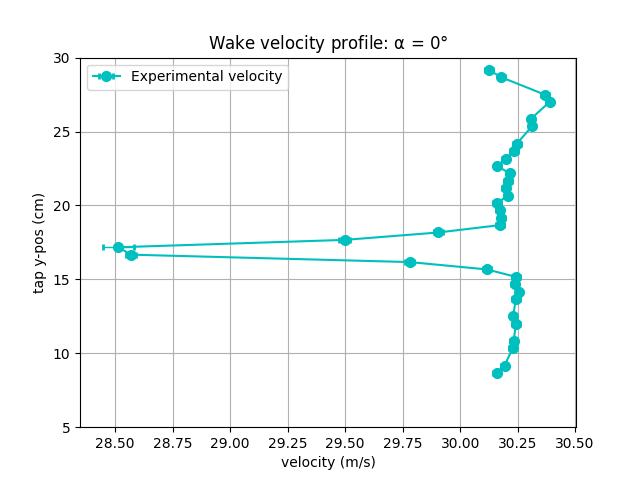
\includegraphics[width=0.8\textwidth]{Figures/vel-graphs/vel-a0.png}
        \caption{Velocity profile for an alpha of 0\degree.}
        \label{fig:vel-a0}
\end{figure}

\begin{figure}[!hpt]
        \centering        
        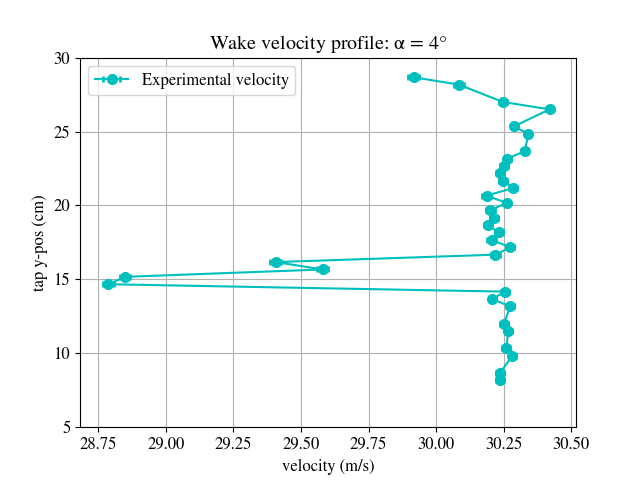
\includegraphics[width=0.8\textwidth]{Figures/vel-graphs/vel-a4.png}
        \caption{Velocity profile for an alpha of 4\degree.}
        \label{fig:vel-a4}
\end{figure}

\begin{figure}[!hpt]
        \centering        
        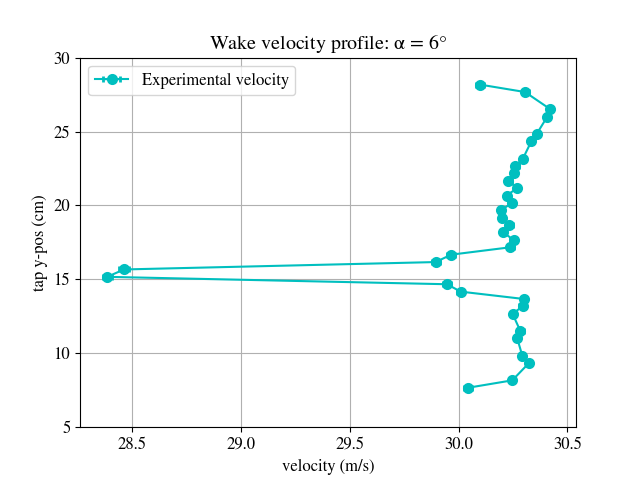
\includegraphics[width=0.8\textwidth]{Figures/vel-graphs/vel-a6.png}
        \caption{Velocity profile for an alpha of 6\degree.}
        \label{fig:vel-a6}
\end{figure}

\begin{figure}[!hpt]
        \centering        
        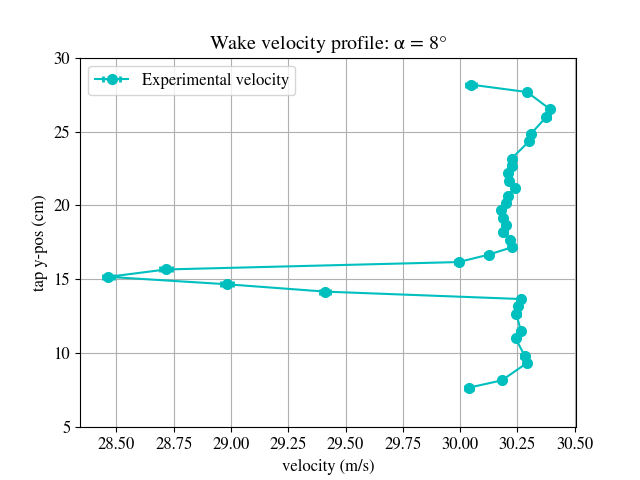
\includegraphics[width=0.8\textwidth]{Figures/vel-graphs/vel-a8.png}
        \caption{Velocity profile for an alpha of 8\degree.}
        \label{fig:vel-a8}
\end{figure}

\begin{figure}[!hpt]
        \centering        
        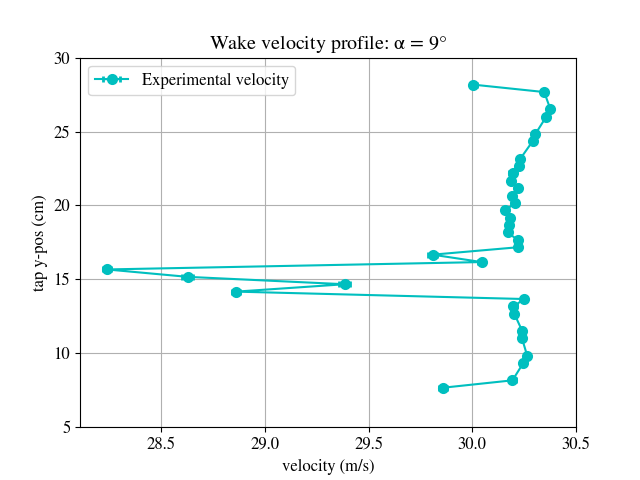
\includegraphics[width=0.8\textwidth]{Figures/vel-graphs/vel-a9.png}
        \caption{Velocity profile for an alpha of 9\degree.}
        \label{fig:vel-a9}
\end{figure}

\begin{figure}[!hpt]
        \centering        
        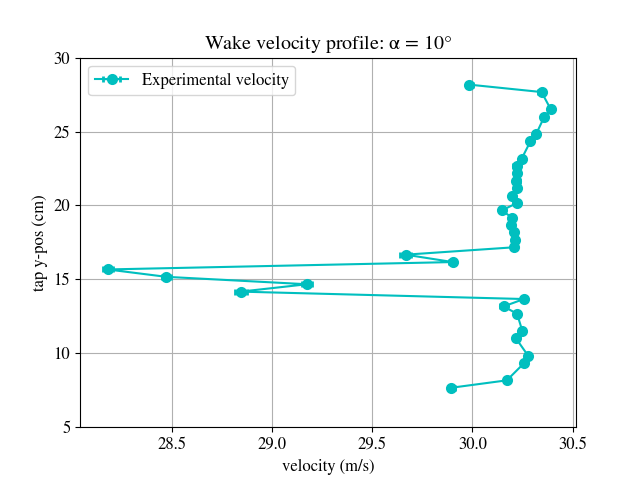
\includegraphics[width=0.8\textwidth]{Figures/vel-graphs/vel-a10.png}
        \caption{Velocity profile for an alpha of 10\degree.}
        \label{fig:vel-a10}
\end{figure}

\begin{figure}[!hpt]
        \centering        
        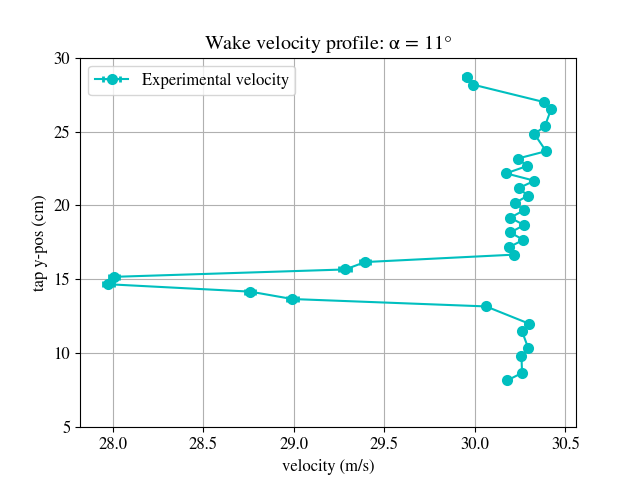
\includegraphics[width=0.8\textwidth]{Figures/vel-graphs/vel-a11.png}
        \caption{Velocity profile for an alpha of 11\degree.}
        \label{fig:vel-a11}
\end{figure}

\begin{figure}[!hpt]
        \centering        
        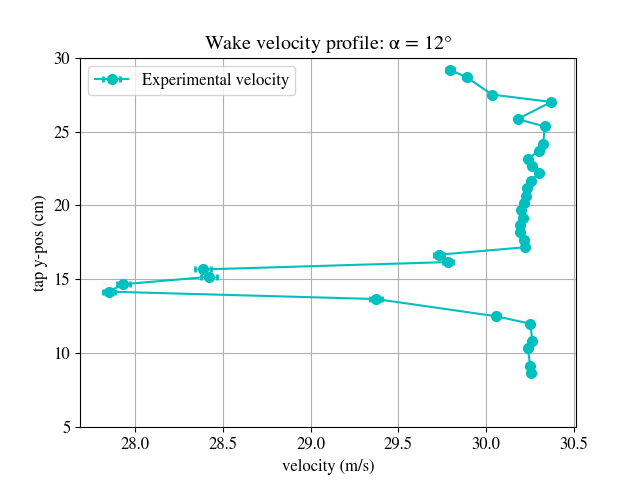
\includegraphics[width=0.8\textwidth]{Figures/vel-graphs/vel-a12.png}
        \caption{Velocity profile for an alpha of 12\degree.}
        \label{fig:vel-a12}
\end{figure}

\begin{figure}[!hpt]
        \centering        
        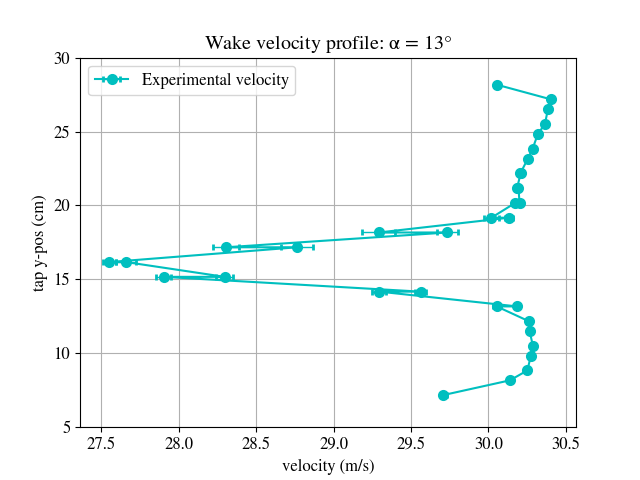
\includegraphics[width=0.8\textwidth]{Figures/vel-graphs/vel-a13.png}
        \caption{Velocity profile for an alpha of 13\degree.}
        \label{fig:vel-a13}
\end{figure}

\begin{figure}[!hpt]
        \centering        
        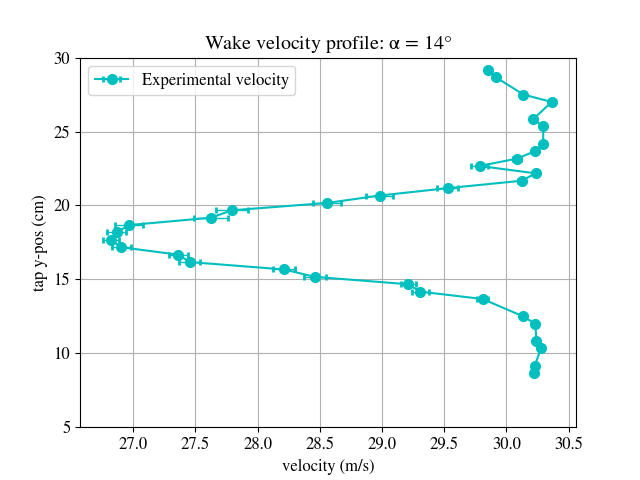
\includegraphics[width=0.8\textwidth]{Figures/vel-graphs/vel-a14.png}
        \caption{Velocity profile for an alpha of 14\degree.}
        \label{fig:vel-a14}
\end{figure}

\begin{figure}[!hpt]
        \centering        
        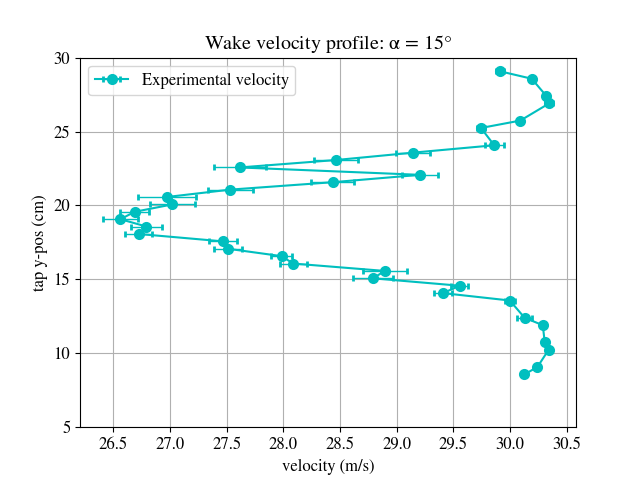
\includegraphics[width=0.8\textwidth]{Figures/vel-graphs/vel-a15.png}
        \caption{Velocity profile for an alpha of 15\degree.}
        \label{fig:vel-a15}
\end{figure}

\begin{figure}[!hpt]
        \centering        
        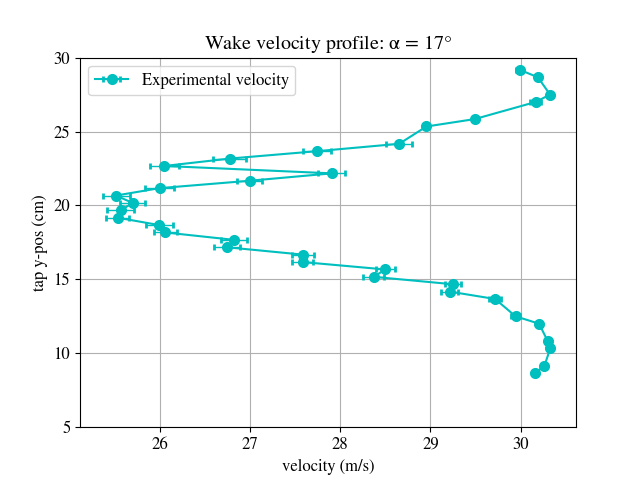
\includegraphics[width=0.8\textwidth]{Figures/vel-graphs/vel-a17.png}
        \caption{Velocity profile for an alpha of 17\degree.}
        \label{fig:vel-a17}
\end{figure}

%%%%% c_p %%%%%%%%%%%%%%%%%%%%%%

\begin{figure}[!hpt]
        \centering        
        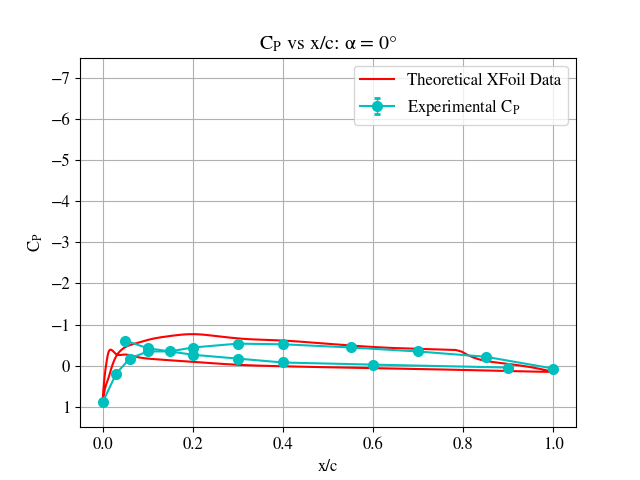
\includegraphics[width=0.8\textwidth]{Figures/C_p-a0.png}
        \caption{Coefficient of pressure over chord for an alpha of 0\degree.}
        \label{fig:C_p-a0}
\end{figure}

\begin{figure}[!hpt]
        \centering        
        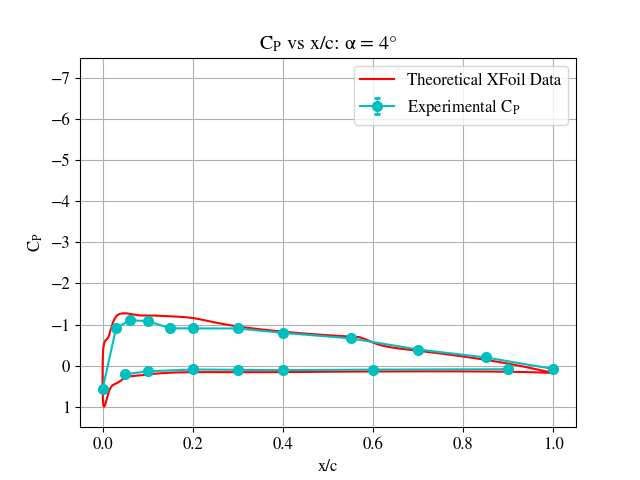
\includegraphics[width=0.8\textwidth]{Figures/C_p-a4.png}
        \caption{Coefficient of pressure over chord for an alpha of 4\degree.}
        \label{fig:C_p-a4}
\end{figure}

\begin{figure}[!hpt]
        \centering        
        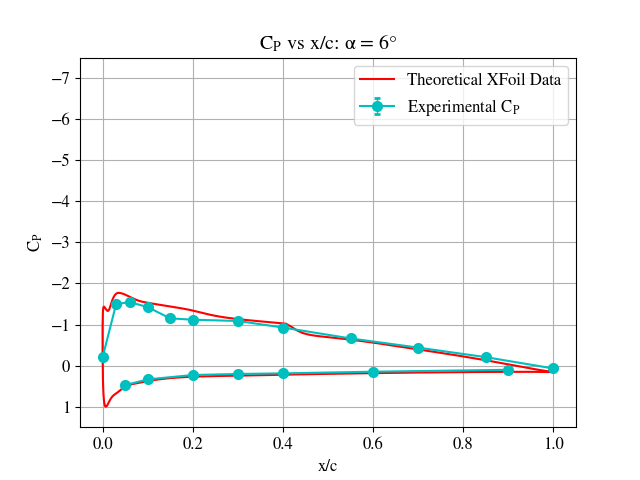
\includegraphics[width=0.8\textwidth]{Figures/C_p-a6.png}
        \caption{Coefficient of pressure over chord for an alpha of 6\degree.}
        \label{fig:C_p-a6}
\end{figure}

\begin{figure}[!hpt]
        \centering        
        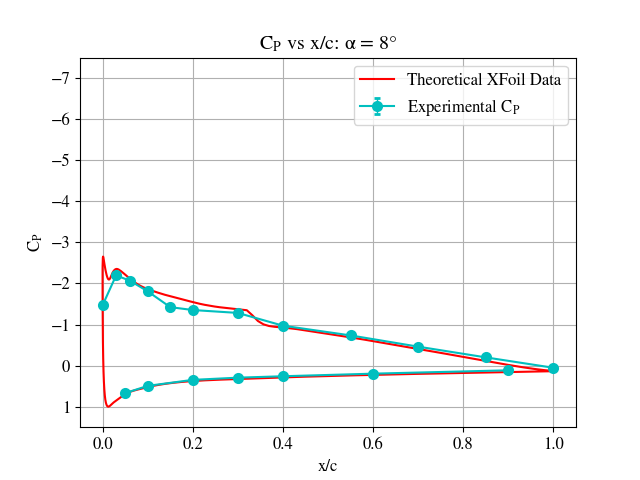
\includegraphics[width=0.8\textwidth]{Figures/C_p-a8.png}
        \caption{Coefficient of pressure over chord for an alpha of 8\degree.}
        \label{fig:C_p-a8}
\end{figure}

\begin{figure}[!hpt]
        \centering        
        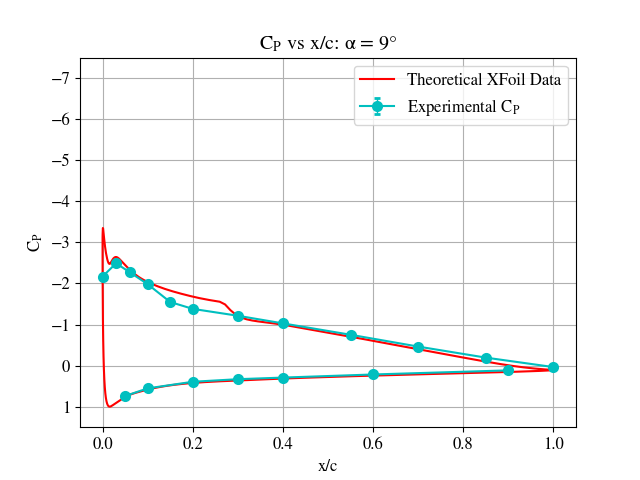
\includegraphics[width=0.8\textwidth]{Figures/C_p-a9.png}
        \caption{Coefficient of pressure over chord for an alpha of 9\degree.}
        \label{fig:C_p-a9}
\end{figure}

\begin{figure}[!hpt]
        \centering        
        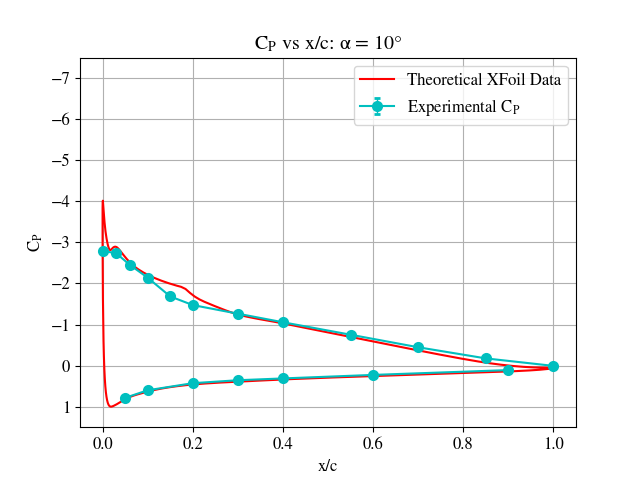
\includegraphics[width=0.8\textwidth]{Figures/C_p-a10.png}
        \caption{Coefficient of pressure over chord for an alpha of 10\degree.}
        \label{fig:C_p-a10}
\end{figure}

\begin{figure}[!hpt]
        \centering        
        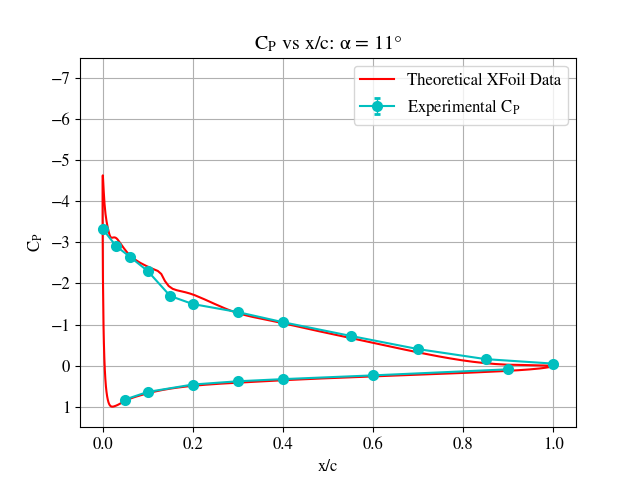
\includegraphics[width=0.8\textwidth]{Figures/C_p-a11.png}
        \caption{Coefficient of pressure over chord for an alpha of 11\degree.}
        \label{fig:C_p-a11}
\end{figure}

\begin{figure}[!hpt]
        \centering        
        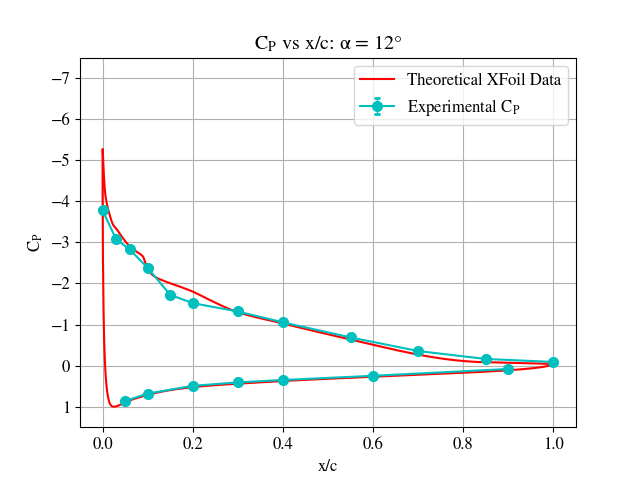
\includegraphics[width=0.8\textwidth]{Figures/C_p-a12.png}
        \caption{Coefficient of pressure over chord for an alpha of 12\degree.}
        \label{fig:C_p-a12}
\end{figure}

\begin{figure}[!hpt]
        \centering        
        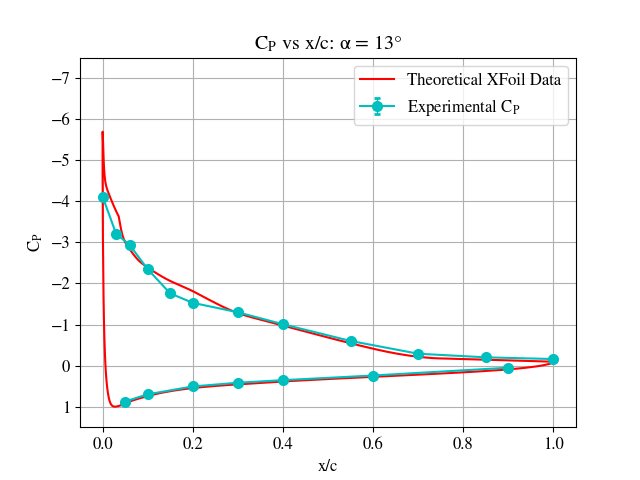
\includegraphics[width=0.8\textwidth]{Figures/C_p-a13.png}
        \caption{Coefficient of pressure over chord for an alpha of 13\degree.}
        \label{fig:C_p-a13}
\end{figure}

\begin{figure}[!hpt]
        \centering        
        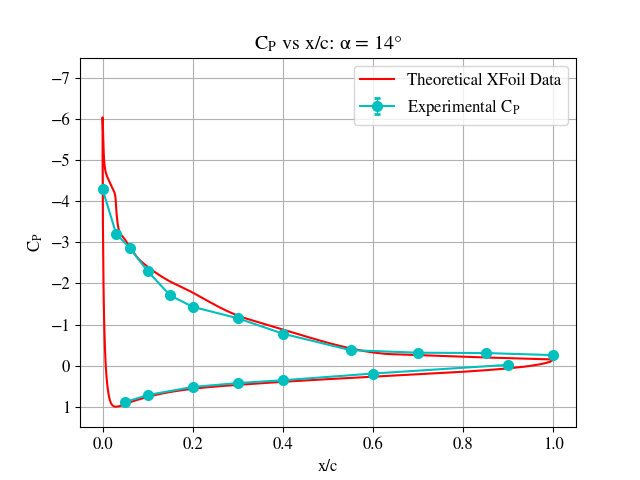
\includegraphics[width=0.8\textwidth]{Figures/C_p-a14.png}
        \caption{Coefficient of pressure over chord for an alpha of 14\degree.}
        \label{fig:C_p-a14}
\end{figure}

\begin{figure}[!hpt]
        \centering        
        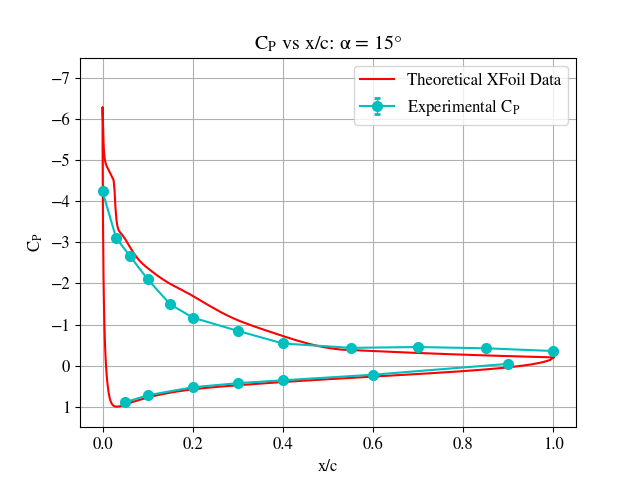
\includegraphics[width=0.8\textwidth]{Figures/C_p-a15.png}
        \caption{Coefficient of pressure over chord for an alpha of 15\degree.}
        \label{fig:C_p-a15}
\end{figure}

\begin{figure}[!hpt]
        \centering        
        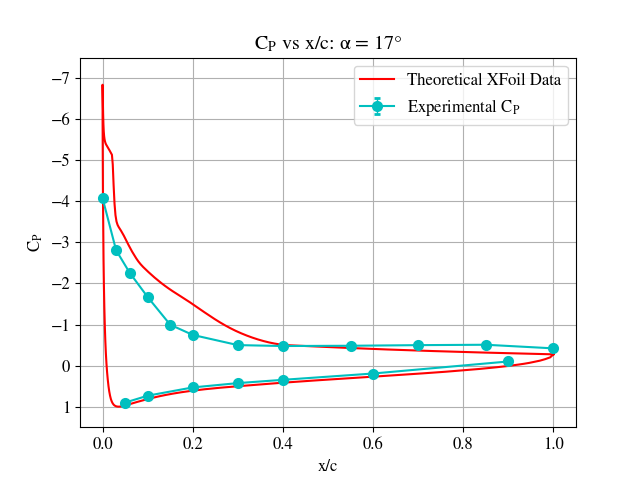
\includegraphics[width=0.8\textwidth]{Figures/C_p-a17.png}
        \caption{Coefficient of pressure over chord for an alpha of 17\degree.}
        \label{fig:C_p-a17}
\end{figure}

%%%%%%%%%%%%%%%%%

\begin{figure}[!hpt]
        \centering        
        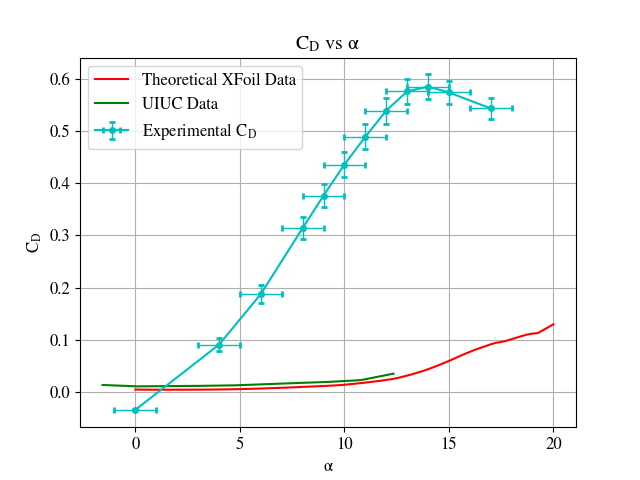
\includegraphics[width=0.8\textwidth]{Figures/C_d-a.png}
        \caption{Coefficient of Drag vs. Angle of Attack.}
        \label{fig:C_d-a}
\end{figure}

\begin{figure}[!hpt]
        \centering        
        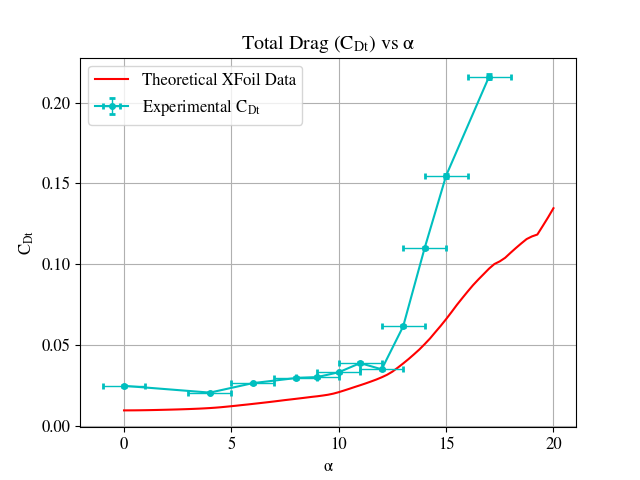
\includegraphics[width=0.8\textwidth]{Figures/C_Dt-a.png}
        \caption{Coefficient of Total Drag vs. Angle of Attack.}
        \label{fig:C_Dt-a}
\end{figure}

\begin{figure}[!hpt]
        \centering        
        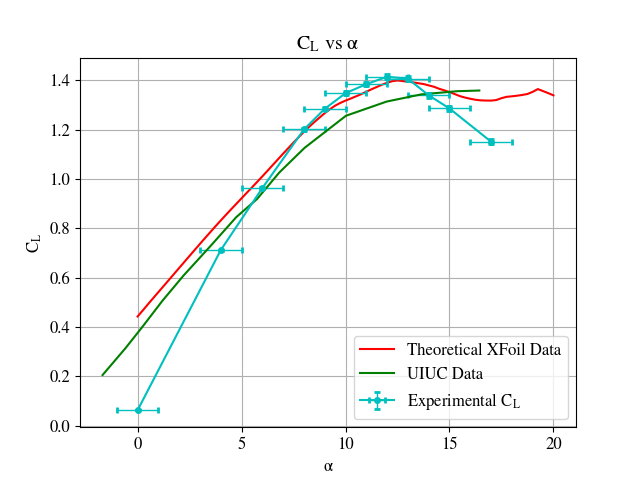
\includegraphics[width=0.8\textwidth]{Figures/C_l-a.png}
        \caption{Coefficient of Lift vs. Angle of Attack.}
        \label{fig:C_p-a17}
\end{figure}

\begin{figure}[!hpt]
        \centering        
        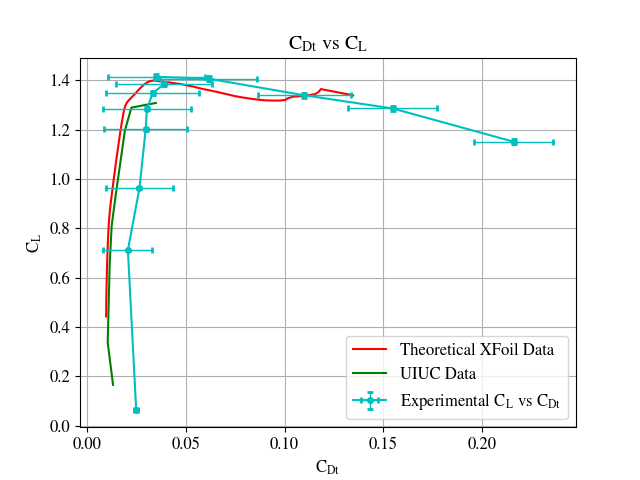
\includegraphics[width=0.8\textwidth]{Figures/C_l-C_d.png}
        \caption{Coefficient of Lift vs. Coefficient of Drag.}
        \label{fig:C_l-C}
\end{figure}

\begin{figure}[!hpt]
        \centering        
        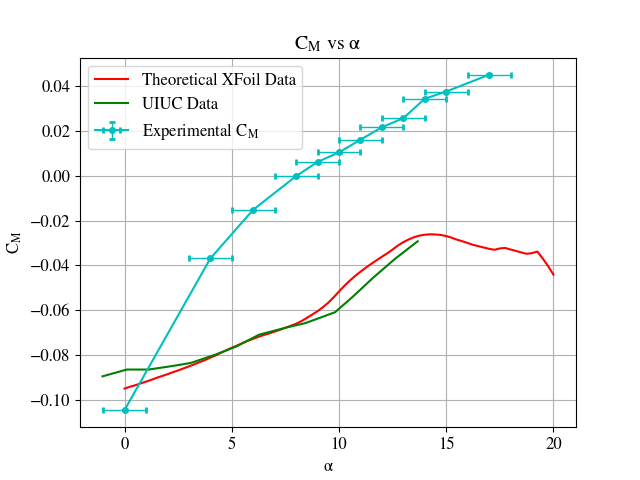
\includegraphics[width=0.8\textwidth]{Figures/C_m-a.png}
        \caption{Coefficient of Moment vs. Angle of Attack.}
        \label{fig:C_m-a}
\end{figure}


\newpage

\section{Raw Pressure Measurements}

\begin{table}[!hpt]
    \caption{Scanivalve airfoil pressure data in pascals from angle of attack 0 to 10 degrees (columns).}
    \centering
    \begin{tabular}{|l|l|l|l|l|l|l|}
    \hline
        ~ & \multicolumn{6}{c|}{Angle of Attack}\\ \hline
        Tap \# & 0\degree (Pa) & 4\degree (Pa) & 6\degree (Pa) & 8\degree (Pa) & 9\degree (Pa) & 10\degree (Pa) \\ \hline
        1 & 532.9035682 & 340.8428824 & -118.0891819 & -873.2776504 & -1288.638426 & -1658.593267 \\ \hline
        2 & 117.8630552 & -542.8765287 & -890.7856597 & -1306.123145 & -1479.769344 & -1627.78351 \\ \hline
        3 & -100.977744 & -654.308017 & -922.2238733 & -1232.29287 & -1351.519361 & -1459.80888 \\ \hline
        4 & -204.8456448 & -644.9190854 & -848.9436297 & -1076.565209 & -1177.458159 & -1272.768652 \\ \hline
        5 & -205.5408773 & -539.2325226 & -685.1525432 & -847.1152394 & -919.9248999 & -1001.098771 \\ \hline
        6 & -342.4246142 & -645.293306 & -772.2527427 & -921.1814044 & -999.1857869 & -1034.088034 \\ \hline
        7 & -317.5447473 & -536.609937 & -647.4073784 & -763.1696371 & -721.0541572 & -751.4383699 \\ \hline
        8 & -308.0369561 & -473.0224947 & -552.6879514 & -578.2709612 & -610.5750725 & -627.3914994 \\ \hline
        9 & -262.5054993 & -393.9555404 & -394.1783692 & -437.3724553 & -446.1828707 & -447.1521672 \\ \hline
        10 & -203.8999689 & -232.3343146 & -260.8423349 & -274.3526416 & -275.1147448 & -265.4806642 \\ \hline
        11 & -127.5357169 & -117.7566046 & -122.4512079 & -119.0154006 & -115.353482 & -104.2628018 \\ \hline
        12 & 43.2740797 & 48.88133552 & 41.93789756 & 31.67029425 & 21.46942776 & 4.086570075 \\ \hline
        13 & 28.45719863 & 52.17141413 & 60.88204168 & 68.28019989 & 69.04691871 & 65.03845873 \\ \hline
        14 & -14.00614968 & 57.91410482 & 88.76972522 & 116.8324737 & 128.4694068 & 134.6946893 \\ \hline
        15 & -44.87517107 & 65.93995188 & 112.5089286 & 154.3569688 & 173.2677102 & 185.6897343 \\ \hline
        16 & -100.9878605 & 61.1222409 & 121.5841062 & 174.8304045 & 196.6791258 & 211.796811 \\ \hline
        17 & -156.989528 & 56.20379694 & 136.6767107 & 206.7180611 & 233.9623806 & 254.5937162 \\ \hline
        18 & -251.4109283 & 82.98294878 & 199.8034958 & 293.7613469 & 329.4820105 & 357.0653116 \\ \hline
        19 & -362.7563795 & 125.6674027 & 283.4808135 & 399.0008799 & 439.2845054 & 466.5315197 \\ \hline
    \end{tabular}
\end{table}

\begin{table}[!hpt]
    \caption{Scanivalve airfoil pressure data in pascals from angle of attack 11 to 17 degrees (columns).}
    \centering
    \begin{tabular}{|l|l|l|l|l|l|l|}
    \hline
        ~ & \multicolumn{6}{c|}{Angle of Attack}\\ \hline
        Tap \# & 11\degree (Pa) & 12\degree (Pa) & 13\degree (Pa) & 14\degree (Pa) & 15\degree (Pa) & 17\degree (Pa) \\ \hline
        1 & -1982.958656 & -2231.643322 & -2446.403958 & -2540.391459 & -2520.873011 & -2416.720063 \\ \hline
        2 & -1731.425351 & -1818.438057 & -1907.982043 & -1902.605731 & -1848.995697 & -1665.71629 \\ \hline
        3 & -1580.040813 & -1670.781228 & -1746.322555 & -1695.995559 & -1593.285689 & -1341.08484 \\ \hline
        4 & -1371.230199 & -1405.982962 & -1395.504303 & -1360.101323 & -1249.329267 & -989.8248244 \\ \hline
        5 & -1008.654389 & -1017.975678 & -1044.819119 & -1011.127293 & -887.620742 & -589.9233604 \\ \hline
        6 & -1041.87476 & -1058.304908 & -1076.039351 & -1009.370806 & -864.4739774 & -468.7534448 \\ \hline
        7 & -775.4321019 & -778.2227323 & -771.7460524 & -682.3218937 & -502.5960348 & -295.7933885 \\ \hline
        8 & -629.0496515 & -622.02666 & -598.447053 & -459.9707256 & -320.4546491 & -282.6070096 \\ \hline
        9 & -430.5679994 & -405.5003636 & -356.862682 & -222.611725 & -257.0863425 & -286.290312 \\ \hline
        10 & -238.7186314 & -209.5259873 & -171.8791428 & -185.4906279 & -268.7958233 & -295.2914274 \\ \hline
        11 & -93.52886861 & -95.48676574 & -119.655342 & -181.0118439 & -250.6447261 & -300.9595505 \\ \hline
        12 & -28.78350575 & -52.2603426 & -94.85539535 & -150.9359428 & -210.9848543 & -248.7933359 \\ \hline
        13 & 53.85043615 & 48.60754768 & 30.60348788 & -11.18206683 & -25.64082838 & -59.66490149 \\ \hline
        14 & 141.7029314 & 146.6481378 & 143.5418955 & 114.2966637 & 132.0591612 & 114.2359278 \\ \hline
        15 & 195.9758842 & 207.0897092 & 210.9097004 & 211.4613507 & 212.8357907 & 205.3146648 \\ \hline
        16 & 226.9802637 & 241.4652489 & 248.2304762 & 251.5646958 & 254.1783507 & 252.7471381 \\ \hline
        17 & 274.5924732 & 291.0866925 & 301.7374972 & 308.2772759 & 313.8601182 & 315.0064139 \\ \hline
        18 & 381.611126 & 402.3294237 & 415.6779919 & 424.2984827 & 430.2571482 & 434.3441358 \\ \hline
        19 & 491.332711 & 509.5248313 & 520.0496436 & 526.2332633 & 530.3437106 & 533.939004 \\ \hline
    \end{tabular}
\end{table}

\begin{table}[!ht]
    \centering
    \caption{Scanivalve wake rake pressure data in pascals and rake position from bottom of test section. From angle of attack 0 to 6 degrees.}
    \begin{tabular}{|l|l|l|l|l|l|}
    \hline
        \multicolumn{2}{|c|}{\alpha = 0} &  
        \multicolumn{2}{c|}{\alpha = 4} & 
        \multicolumn{2}{c|}{\alpha = 6} \\ \hline
        y Pos (cm) & Pressure (Pa) & y Pos (cm) & Pressure (Pa) & y Pos (cm) & Pressure (Pa) \\ \hline
        8.67 & 557.0874069 & 8.17 & 560.008693 & 7.67 & 552.8708145 \\ \hline
        9.17 & 558.3791119 & 8.67 & 559.9901598 & 8.17 & 560.3613694 \\ \hline
        10.34 & 559.6737966 & 9.84 & 561.6714594 & 9.34 & 563.204516 \\ \hline
        10.84 & 559.8214676 & 10.34 & 560.8320629 & 9.84 & 562.0621551 \\ \hline
        12 & 560.2245558 & 11.5 & 561.1144258 & 11 & 561.211788 \\ \hline
        12.5 & 559.7512818 & 12 & 560.5379947 & 11.5 & 561.7484651 \\ \hline
        13.67 & 560.1895349 & 13.17 & 561.3622659 & 12.67 & 560.4020371 \\ \hline
        14.17 & 560.6976857 & 13.67 & 558.917353 & 13.17 & 562.1080169 \\ \hline
        14.67 & 559.9997207 & 14.17 & 560.641693 & 13.67 & 562.3843112 \\ \hline
        15.17 & 560.1640851 & 14.67 & 507.5694927 & 14.17 & 551.6031867 \\ \hline
        15.67 & 555.5877558 & 15.17 & 509.7968123 & 14.67 & 549.2803777 \\ \hline
        16.17 & 543.2050249 & 15.67 & 535.9464952 & 15.17 & 493.4432441 \\ \hline
        16.67 & 499.9531275 & 16.17 & 529.6501535 & 15.67 & 496.1641716 \\ \hline
        17.17 & 497.941288 & 16.67 & 559.3292138 & 16.17 & 547.369625 \\ \hline
        17.67 & 532.9550417 & 17.17 & 561.4040325 & 16.67 & 549.9959746 \\ \hline
        18.17 & 547.7359843 & 17.67 & 558.8104094 & 17.17 & 560.0160376 \\ \hline
        18.67 & 557.6340729 & 18.17 & 559.8187224 & 17.67 & 560.6098433 \\ \hline
        19.17 & 557.8662258 & 18.67 & 558.2711249 & 18.17 & 558.8033632 \\ \hline
        19.67 & 557.5608929 & 19.17 & 559.1677674 & 18.67 & 559.882177 \\ \hline
        20.17 & 557.2282848 & 19.67 & 558.6331173 & 19.17 & 558.6683111 \\ \hline
        20.67 & 558.8601276 & 20.17 & 560.8755252 & 19.67 & 558.3925745 \\ \hline
        21.17 & 558.5766554 & 20.67 & 558.1320949 & 20.17 & 560.3344977 \\ \hline
        21.67 & 558.9084424 & 21.17 & 561.7892583 & 20.67 & 559.3785575 \\ \hline
        22.17 & 559.2143433 & 21.67 & 560.421873 & 21.17 & 561.1926888 \\ \hline
        22.67 & 557.1662317 & 22.17 & 559.9456295 & 21.67 & 559.6341435 \\ \hline
        23.17 & 558.5974935 & 22.67 & 560.5143045 & 22.17 & 560.7260186 \\ \hline
        23.67 & 559.9109646 & 23.17 & 560.9886424 & 22.67 & 560.8987894 \\ \hline
        24.17 & 560.3340326 & 23.67 & 563.3713787 & 23.17 & 562.1775977 \\ \hline
        25.34 & 804.0764393 & 24.84 & 805.4912318 & 24.34 & 805.3145695 \\ \hline
        25.84 & 805.3385108 & 25.34 & 805.933825 & 24.84 & 805.6286093 \\ \hline
        27 & 565.6289387 & 26.5 & 566.7864332 & 26 & 566.3353431 \\ \hline
        27.5 & 564.8374453 & 27 & 560.3702471 & 26.5 & 566.8856907 \\ \hline
        28.67 & 557.8607375 & 28.17 & 554.3557559 & 27.67 & 562.5388493 \\ \hline
        29.17 & 555.810461 & 28.67 & 548.214191 & 28.17 & 554.9290323 \\ \hline
    \end{tabular}
\end{table}

\begin{table}[!ht]
    \centering
    \caption{Scanivalve wake rake pressure data in pascals and rake position from bottom of test section. From angle of attack 8 to 10 degrees.}
    \begin{tabular}{|l|l|l|l|l|l|}
    \hline
        \multicolumn{2}{|c|}{\alpha = 8\degree} &  
        \multicolumn{2}{c|}{\alpha = 9\degree} & 
        \multicolumn{2}{c|}{\alpha = 10\degree} \\ \hline
        y Pos (cm) & Pressure (Pa) & y Pos (cm) & Pressure (Pa) & y Pos (cm) & Pressure (Pa) \\ \hline
        7.67 & 552.6227789 & 7.67 & 546.0771402 & 7.67 & 547.4064343 \\ \hline
        8.17 & 557.9606432 & 8.17 & 558.4231277 & 8.17 & 557.5692396 \\ \hline
        9.34 & 562.0254941 & 9.34 & 560.3565561 & 9.34 & 560.7676884 \\ \hline
        9.84 & 561.6391014 & 9.84 & 561.0538935 & 9.84 & 561.4870142 \\ \hline
        11 & 560.204899 & 11 & 560.1279695 & 11 & 559.2640739 \\ \hline
        11.5 & 561.0589476 & 11.5 & 560.1792743 & 11.5 & 560.4352121 \\ \hline
        12.67 & 560.2961863 & 12.67 & 558.7541738 & 12.67 & 559.4557155 \\ \hline
        13.17 & 560.5019366 & 13.17 & 558.5863912 & 13.17 & 556.9763558 \\ \hline
        13.67 & 561.0487652 & 13.67 & 560.5274954 & 13.67 & 560.7168816 \\ \hline
        14.17 & 529.8482671 & 14.17 & 510.1580968 & 14.17 & 509.5704996 \\ \hline
        14.67 & 514.4286714 & 14.67 & 528.8692025 & 14.67 & 521.3321828 \\ \hline
        15.17 & 496.2595561 & 15.17 & 501.9386592 & 15.17 & 496.5889683 \\ \hline
        15.67 & 505.1126029 & 15.67 & 488.3788589 & 15.67 & 486.3938088 \\ \hline
        16.17 & 551.0073704 & 16.17 & 552.921786 & 16.17 & 547.6440796 \\ \hline
        16.67 & 555.8218122 & 16.67 & 544.2560923 & 16.67 & 539.0538955 \\ \hline
        17.17 & 559.5941384 & 17.17 & 559.3499819 & 17.17 & 558.9213802 \\ \hline
        17.67 & 559.328827 & 17.67 & 559.3461069 & 17.67 & 559.0271467 \\ \hline
        18.17 & 558.2125023 & 18.17 & 557.5533466 & 18.17 & 558.8226187 \\ \hline
        18.67 & 558.64523 & 18.67 & 557.8277127 & 18.67 & 558.353693 \\ \hline
        19.17 & 558.1935534 & 19.17 & 557.9651355 & 19.17 & 558.5203438 \\ \hline
        19.67 & 557.8026108 & 19.67 & 557.1581196 & 19.67 & 556.6474128 \\ \hline
        20.17 & 558.6596577 & 20.17 & 558.8856473 & 20.17 & 559.4920637 \\ \hline
        20.67 & 558.8783809 & 20.67 & 558.4008039 & 20.67 & 558.4506271 \\ \hline
        21.17 & 560.0392504 & 21.17 & 559.4043036 & 21.17 & 559.4468851 \\ \hline
        21.67 & 559.1193066 & 21.67 & 558.1283969 & 21.67 & 559.3258348 \\ \hline
        22.17 & 559.0371562 & 22.17 & 558.4686232 & 22.17 & 559.4241642 \\ \hline
        22.67 & 559.5619882 & 22.67 & 559.5900082 & 22.67 & 559.3828338 \\ \hline
        23.17 & 559.5423952 & 23.17 & 559.8479586 & 23.17 & 560.31239 \\ \hline
        24.34 & 803.2395925 & 24.34 & 802.4437324 & 24.34 & 802.9875523 \\ \hline
        24.84 & 803.3965219 & 24.84 & 803.2180116 & 24.84 & 803.5620614 \\ \hline
        26 & 565.1802028 & 26 & 564.4641346 & 26 & 564.4900576 \\ \hline
        26.5 & 565.802473 & 26.5 & 565.2270667 & 26.5 & 565.6991204 \\ \hline
        27.67 & 562.0367815 & 27.67 & 564.1000967 & 27.67 & 563.9770276 \\ \hline
        28.17 & 553.012172 & 28.17 & 551.4833134 & 28.17 & 550.7025231 \\ \hline
    \end{tabular}
\end{table}

\begin{table}[!ht]
    \caption{Scanivalve wake rake pressure data in pascals and rake position from bottom of test section. From angle of attack 11 to 13 degrees.}
    \centering
    \begin{tabular}{|l|l|l|l|l|l|}
    \hline
        \multicolumn{2}{|c|}{\alpha = 11\degree} &  
        \multicolumn{2}{c|}{\alpha = 12\degree} & 
        \multicolumn{2}{c|}{\alpha = 13\degree} \\ \hline
        y Pos (cm) & Pressure (Pa) & y Pos (cm) & Pressure (Pa) & y Pos (cm) & Pressure (Pa) \\ \hline
        8.17 & 557.8589615 & 8.67 & 560.7664805 & 7.17 & 540.5427181 \\ \hline
        8.67 & 560.8686971 & 9.17 & 560.5396986 & 8.17 & 556.3575345 \\ \hline
        9.84 & 560.744881 & 10.34 & 560.0177435 & 8.84 & 560.5251886 \\ \hline
        10.34 & 562.1471762 & 10.84 & 560.9970262 & 9.84 & 561.3705262 \\ \hline
        11.5 & 560.8472459 & 12 & 560.5612981 & 10.5 & 561.8461009 \\ \hline
        12 & 562.3262956 & 12.5 & 553.4317066 & 11.5 & 561.0689201 \\ \hline
        13.17 & 553.5156021 & 13.67 & 528.4236234 & 12.17 & 560.8593276 \\ \hline
        13.67 & 514.81734 & 14.17 & 474.9606712 & 13.17 & 553.2116376 \\ \hline
        14.17 & 506.6112354 & 14.67 & 477.855948 & 13.17 & 558.1018689 \\ \hline
        14.67 & 479.3725971 & 15.17 & 494.6582686 & 14.17 & 525.6244844 \\ \hline
        15.17 & 480.4198102 & 15.67 & 493.4814794 & 14.17 & 535.2408399 \\ \hline
        15.67 & 525.273123 & 16.17 & 543.3596947 & 15.17 & 476.8229095 \\ \hline
        16.17 & 529.1819788 & 16.67 & 541.4532883 & 15.17 & 490.4184386 \\ \hline
        16.67 & 559.1240006 & 17.17 & 559.38405 & 16.17 & 468.5567477 \\ \hline
        17.17 & 558.1473047 & 17.67 & 559.2595548 & 16.17 & 464.9430527 \\ \hline
        17.67 & 561.1458702 & 18.17 & 558.3539441 & 17.17 & 506.7590709 \\ \hline
        18.17 & 558.4538518 & 18.67 & 558.3572799 & 17.17 & 490.7167707 \\ \hline
        18.67 & 561.2936626 & 19.17 & 558.9892386 & 18.17 & 541.5136025 \\ \hline
        19.17 & 558.4556339 & 19.67 & 558.6174734 & 18.17 & 525.5072946 \\ \hline
        19.67 & 561.2439155 & 20.17 & 559.2187183 & 19.17 & 556.1106843 \\ \hline
        20.17 & 559.4676079 & 20.67 & 559.6412472 & 19.17 & 551.9492511 \\ \hline
        20.67 & 562.0642006 & 21.17 & 559.953793 & 20.17 & 557.6184413 \\ \hline
        21.17 & 560.1651244 & 21.67 & 560.6755657 & 20.17 & 558.6529614 \\ \hline
        21.67 & 563.4188786 & 22.17 & 562.3424437 & 21.17 & 558.4021621 \\ \hline
        22.17 & 557.5884787 & 22.67 & 560.8659128 & 21.17 & 558.0407788 \\ \hline
        22.67 & 561.9284056 & 23.17 & 560.1039746 & 22.17 & 558.9375345 \\ \hline
        23.17 & 559.9711059 & 23.67 & 562.2940014 & 22.17 & 558.8473832 \\ \hline
        23.67 & 565.7954331 & 24.17 & 563.2642396 & 23.17 & 560.6546391 \\ \hline
        24.84 & 803.3156845 & 25.34 & 803.7629696 & 23.84 & 804.1070811 \\ \hline
        25.34 & 812.3927878 & 25.84 & 803.2307869 & 24.84 & 802.7786205 \\ \hline
        26.5 & 566.8053574 & 27 & 564.9892259 & 25.5 & 564.7303124 \\ \hline
        27 & 565.2791783 & 27.5 & 552.495483 & 26.5 & 565.4495126 \\ \hline
        28.17 & 550.8947429 & 28.67 & 547.175728 & 27.17 & 566.2551868 \\ \hline
        28.67 & 549.568122 & 29.17 & 543.7351641 & 28.17 & 553.1932422 \\ \hline
    \end{tabular}
\end{table}

\begin{table}[!ht]
    \caption{Scanivalve wake rake pressure data in pascals and rake position from bottom of test section. From angle of attack 14  to 17 degrees.}
    \centering
    \begin{tabular}{|l|l|l|l|l|l|}
    \hline
        \multicolumn{2}{|c|}{\alpha = 14\degree} &  
        \multicolumn{2}{c|}{\alpha = 15\degree} & 
        \multicolumn{2}{c|}{\alpha = 17\degree} \\ \hline
        y Pos (cm) & Pressure (Pa) & y Pos (cm) & Pressure (Pa) & y Pos (cm) & Pressure (Pa) \\ \hline
        8.67 & 559.29615 & 8.57 & 555.8673468 & 8.67 & 557.2925646 \\ \hline
        9.17 & 559.6950215 & 9.07 & 560.1522194 & 9.17 & 561.0168085 \\ \hline
        10.34 & 561.5211626 & 10.24 & 563.8172233 & 10.34 & 563.4241879 \\ \hline
        10.84 & 560.1675691 & 10.74 & 562.5368737 & 10.84 & 562.2851792 \\ \hline
        12 & 559.8382064 & 11.9 & 561.9066004 & 12 & 558.7935348 \\ \hline
        12.5 & 556.1623822 & 12.4 & 555.979787 & 12.5 & 549.1901172 \\ \hline
        13.67 & 544.2858121 & 13.57 & 551.1584924 & 13.67 & 540.9494918 \\ \hline
        14.17 & 526.1370658 & 14.07 & 529.7161041 & 14.17 & 522.8087794 \\ \hline
        14.67 & 522.5959356 & 14.57 & 535.0384088 & 14.67 & 523.9756044 \\ \hline
        15.17 & 496.1138791 & 15.07 & 507.7330278 & 15.17 & 493.074656 \\ \hline
        15.67 & 487.5423268 & 15.57 & 511.3803752 & 15.67 & 497.4641696 \\ \hline
        16.17 & 461.6848944 & 16.07 & 483.1885913 & 16.17 & 466.097524 \\ \hline
        16.67 & 458.644235 & 16.57 & 479.6759853 & 16.67 & 466.2342388 \\ \hline
        17.17 & 443.3856635 & 17.07 & 463.5984436 & 17.17 & 438.204971 \\ \hline
        17.67 & 440.6080374 & 17.57 & 462.1073883 & 17.67 & 440.7889511 \\ \hline
        18.17 & 442.1351571 & 18.07 & 437.4208243 & 18.17 & 416.1175206 \\ \hline
        18.67 & 445.4039112 & 18.57 & 439.701591 & 18.67 & 413.9250592 \\ \hline
        19.17 & 467.4336977 & 19.07 & 432.1903499 & 19.17 & 399.3534511 \\ \hline
        19.67 & 473.1329885 & 19.57 & 436.3057342 & 19.67 & 400.476005 \\ \hline
        20.17 & 499.6280387 & 20.07 & 447.2388927 & 20.17 & 404.5613011 \\ \hline
        20.67 & 514.4765662 & 20.57 & 445.6015615 & 20.67 & 398.7977406 \\ \hline
        21.17 & 534.0492339 & 21.07 & 464.2962191 & 21.17 & 414.0318771 \\ \hline
        21.67 & 555.7326692 & 21.57 & 495.1979539 & 21.67 & 446.4062788 \\ \hline
        22.17 & 559.9612158 & 22.07 & 522.4190672 & 22.17 & 477.0924617 \\ \hline
        22.67 & 543.3624728 & 22.57 & 467.0983914 & 22.67 & 415.7534145 \\ \hline
        23.17 & 554.4307284 & 23.07 & 496.183404 & 23.17 & 439.1386324 \\ \hline
        23.67 & 559.7610032 & 23.57 & 520.1950897 & 23.67 & 471.5087822 \\ \hline
        24.17 & 562.1418956 & 24.07 & 546.1264117 & 24.17 & 502.8987929 \\ \hline
        25.34 & 803.1542587 & 25.24 & 800.147824 & 25.34 & 802.1153554 \\ \hline
        25.84 & 802.0293177 & 25.74 & 803.8491101 & 25.84 & 803.0109771 \\ \hline
        27 & 564.7039428 & 26.9 & 563.9676806 & 27 & 557.4313558 \\ \hline
        27.5 & 556.3224992 & 27.4 & 563.0816527 & 27.5 & 563.2954719 \\ \hline
        28.67 & 548.1323741 & 28.57 & 558.2961877 & 28.67 & 558.3107698 \\ \hline
        29.17 & 545.6985222 & 29.07 & 548.072992 & 29.17 & 550.9261008 \\ \hline
    \end{tabular}
\end{table}

\begin{table}[!ht]
    \centering
    \caption{Airfoil pressure data uncertainties in pascals from angle of attack 0 to 10 degrees.}
    \begin{tabular}{|l|l|l|l|l|l|l|}
    \hline
        ~ & \multicolumn{6}{c|}{Angle of Attack}\\ \hline
        Tap \# & 0\degree (Pa) & 4\degree (Pa) & 6\degree (Pa) & 8\degree (Pa) & 9\degree (Pa) & 10\degree (Pa) \\ \hline
        1 & 0.2877822 & 0.821539414 & 0.892489337 & 23.35070395 & 1.578263738 & 3.006472342 \\ \hline
        2 & 0.720298076 & 1.400454681 & 1.635520021 & 1.99652191 & 1.416550253 & 3.458252492 \\ \hline
        3 & 0.983215107 & 1.933804133 & 1.724845605 & 1.835345075 & 1.824530133 & 2.44040358 \\ \hline
        4 & 0.960942125 & 2.749560157 & 1.497908797 & 2.538687007 & 2.057682683 & 2.043439264 \\ \hline
        5 & 0.890878239 & 1.406557861 & 2.004043616 & 2.477837802 & 1.628083905 & 1.975977193 \\ \hline
        6 & 1.383792257 & 1.830531151 & 2.674370279 & 1.507817845 & 2.259403355 & 1.918005502 \\ \hline
        7 & 0.919551669 & 1.477276521 & 1.885135206 & 1.576410458 & 1.158648122 & 1.707917318 \\ \hline
        8 & 1.076203463 & 1.432017687 & 1.74441717 & 1.832483499 & 1.995271469 & 1.716500306 \\ \hline
        9 & 1.706740738 & 1.072183637 & 1.427782935 & 1.020278451 & 1.20371086 & 2.327049647 \\ \hline
        10 & 0.853070754 & 1.266756871 & 1.03349001 & 1.562716168 & 1.398561052 & 1.243895431 \\ \hline
        11 & 1.411742673 & 0.759903732 & 0.58090892 & 0.805421807 & 0.670345951 & 0.91768258 \\ \hline
        12 & 0.89566707 & 0.429026374 & 0.655714631 & 0.864204794 & 0.772436864 & 0.764452461 \\ \hline
        13 & 0.474818164 & 0.788874192 & 0.709633505 & 1.257620615 & 0.802701635 & 0.829784139 \\ \hline
        14 & 0.997370078 & 1.374139908 & 0.729451316 & 0.570364206 & 0.417040819 & 0.418229324 \\ \hline
        15 & 0.705929945 & 1.426097728 & 0.59514055 & 0.568075402 & 0.37087995 & 0.421639802 \\ \hline
        16 & 1.217486786 & 0.668106713 & 0.700940752 & 0.725732929 & 0.380080796 & 0.676863984 \\ \hline
        17 & 0.810169658 & 0.656837283 & 0.56197886 & 0.385877604 & 0.502680053 & 0.43977576 \\ \hline
        18 & 0.959493064 & 1.218039364 & 0.380079212 & 0.576730464 & 0.312386888 & 0.340594732 \\ \hline
        19 & 1.310414729 & 1.411419452 & 0.361529619 & 0.333285519 & 0.299089308 & 0.286988505 \\ \hline
    \end{tabular}
\end{table}

\begin{table}[!ht]
    \centering
    \caption{Airfoil pressure data uncertainties in pascals from angle of attack 11 to 17 degrees.}
    \begin{tabular}{|l|l|l|l|l|l|l|l|l|l|l|l|l|l|l|l|l|l|l|l|}
    \hline
        ~ & \multicolumn{6}{c|}{Angle of Attack}\\ \hline
        Tap \# & 11\degree (Pa) & 12\degree (Pa) & 13\degree (Pa) & 14\degree (Pa) & 15\degree (Pa) & 17\degree (Pa) \\ \hline
        1 & 2.769474024 & 2.335740539 & 2.840193104 & 3.153594881 & 10.60998943 & 7.755622989  \\ \hline
        2 & 3.021138618 & 3.345851505 & 2.385927581 & 2.588747745 & 17.41945111 & 6.753406695  \\ \hline
        3 & 2.269458749 & 1.734386236 & 2.915954498 & 3.133069728 & 6.641119895 & 4.792829329  \\ \hline
        4 & 1.748889045 & 1.622547306 & 2.00154697 & 2.082301386 & 8.061889402 & 5.004638104  \\ \hline
        5 & 1.787639128 & 1.664833319 & 1.318765969 & 2.458932601 & 4.486892695 & 7.116275993  \\ \hline
        6 & 2.382446607 & 1.626952219 & 2.858815039 & 2.333386574 & 5.3411119 & 9.760411895  \\ \hline
        7 & 0.825901355 & 1.830633341 & 1.442871792 & 3.734233756 & 9.03805049 & 2.869267134  \\ \hline
        8 & 3.126187661 & 1.197119722 & 1.788395792 & 2.816142562 & 9.781049143 & 2.764557942  \\ \hline
        9 & 2.183989996 & 1.507194311 & 1.806769929 & 1.985187117 & 8.038256808 & 0.977271663  \\ \hline
        10 & 0.915035156 & 1.26591954 & 1.811500121 & 1.665531268 & 8.684808375 & 1.419813439  \\ \hline
        11 & 1.252285308 & 0.456813088 & 1.073168812 & 1.786785987 & 7.269404247 & 1.493713707  \\ \hline
        12 & 0.804966017 & 0.746972092 & 0.834996702 & 1.013008863 & 8.754630056 & 1.769719035  \\ \hline
        13 & 0.632530513 & 0.624549678 & 0.718292153 & 1.126074485 & 1.743716445 & 0.927059844  \\ \hline
        14 & 0.401201685 & 0.676397758 & 0.395094245 & 1.007617824 & 0.887507709 & 0.405794168  \\ \hline
        15 & 0.334161045 & 0.349859624 & 0.357057607 & 0.421359359 & 0.986449723 & 0.772523466  \\ \hline
        16 & 0.297163425 & 0.82407074 & 0.31853218 & 0.573501895 & 1.432581197 & 0.438675458  \\ \hline
        17 & 0.606861271 & 0.320316408 & 0.362552465 & 0.326787844 & 1.332709062 & 0.566833574  \\ \hline
        18 & 0.283367134 & 0.291986338 & 0.265420837 & 0.331482066 & 0.572185204 & 0.396086512  \\ \hline
        19 & 0.299604547 & 0.300705746 & 0.26410304 & 0.311200132 & 0.473103459 & 0.351365091  \\ \hline
    \end{tabular}
\end{table}

\begin{table}[!ht]
    \centering
    \caption{Wake rake pressure data uncertainties in pascals from angle of attack 0 to 6 degrees.}
    \begin{tabular}{|l|l|l|l|l|l|}
    
    \hline
        \multicolumn{2}{|c|}{\alpha = 0} &  
        \multicolumn{2}{c|}{\alpha = 4} & 
        \multicolumn{2}{c|}{\alpha = 6} \\ \hline
        y Pos (cm) & Uncertainty (Pa) & y Pos (cm) & Uncertainty (Pa) & y Pos (cm) & Uncertainty (Pa) \\ \hline
        8.67 & 0.567045949 & 8.17 & 0.546520149 & 7.67 & 0.643534181 \\ \hline
        9.17 & 0.582713036 & 8.67 & 0.540846108 & 8.17 & 0.500078895 \\ \hline
        10.34 & 0.584292301 & 9.84 & 0.510611032 & 9.34 & 0.495044469 \\ \hline
        10.84 & 0.579334861 & 10.34 & 0.533237957 & 9.84 & 0.502217459 \\ \hline
        12 & 0.611026391 & 11.5 & 0.48878908 & 11 & 0.469011073 \\ \hline
        12.5 & 0.499981719 & 12 & 0.548054643 & 11.5 & 0.597599137 \\ \hline
        13.67 & 0.624527036 & 13.17 & 0.524595718 & 12.67 & 0.50931841 \\ \hline
        14.17 & 0.525405254 & 13.67 & 0.48546328 & 13.17 & 0.523882671 \\ \hline
        14.67 & 0.531766956 & 14.17 & 0.542969155 & 13.67 & 0.497892486 \\ \hline
        15.17 & 0.613207126 & 14.67 & 0.710230321 & 14.17 & 0.605988591 \\ \hline
        15.67 & 0.626798936 & 15.17 & 0.642551971 & 14.67 & 0.623803109 \\ \hline
        16.17 & 0.664918125 & 15.67 & 0.735962535 & 15.17 & 0.682308582 \\ \hline
        16.67 & 0.694199113 & 16.17 & 0.751698819 & 15.67 & 0.717246909 \\ \hline
        17.17 & 2.222763981 & 16.67 & 0.580073828 & 16.17 & 0.663774896 \\ \hline
        17.67 & 0.834381094 & 17.17 & 0.521101525 & 16.67 & 0.68351523 \\ \hline
        18.17 & 0.7192227 & 17.67 & 0.554917789 & 17.17 & 0.555556375 \\ \hline
        18.67 & 0.578952725 & 18.17 & 0.544102949 & 17.67 & 0.569823424 \\ \hline
        19.17 & 0.578466902 & 18.67 & 0.474707962 & 18.17 & 0.536308582 \\ \hline
        19.67 & 0.562011286 & 19.17 & 0.503234496 & 18.67 & 0.53640465 \\ \hline
        20.17 & 0.630319159 & 19.67 & 0.60159714 & 19.17 & 0.527249481 \\ \hline
        20.67 & 0.570869033 & 20.17 & 0.504188037 & 19.67 & 0.502694599 \\ \hline
        21.17 & 0.57165698 & 20.67 & 0.577947192 & 20.17 & 0.543095971 \\ \hline
        21.67 & 0.618520548 & 21.17 & 0.556589475 & 20.67 & 0.489232321 \\ \hline
        22.17 & 0.541851236 & 21.67 & 0.52191097 & 21.17 & 0.489211963 \\ \hline
        22.67 & 0.555395936 & 22.17 & 0.556417464 & 21.67 & 0.597363941 \\ \hline
        23.17 & 0.554435738 & 22.67 & 0.516038486 & 22.17 & 0.498940828 \\ \hline
        23.67 & 0.59483736 & 23.17 & 0.51201294 & 22.67 & 0.541445321 \\ \hline
        24.17 & 0.632008932 & 23.67 & 0.51542996 & 23.17 & 0.496572114 \\ \hline
        25.34 & 0.05500125 & 24.84 & 0.10176055 & 24.34 & 0.178282809 \\ \hline
        25.84 & 0.096686148 & 25.34 & 0.176037661 & 24.84 & 0.110436973 \\ \hline
        27 & 0.637858089 & 26.5 & 0.540823184 & 26 & 0.490815344 \\ \hline
        27.5 & 0.655458688 & 27 & 0.567897821 & 26.5 & 0.512439851 \\ \hline
        28.67 & 0.571066548 & 28.17 & 0.632190693 & 27.67 & 0.592928016 \\ \hline
        29.17 & 0.620454948 & 28.67 & 0.743943164 & 28.17 & 0.678623484 \\ \hline
    \end{tabular}
\end{table}

\begin{table}[!ht]
    \centering
    \caption{Wake rake pressure data uncertainties in pascals from angle of attack 8 to 10 degrees.}
    \begin{tabular}{|l|l|l|l|l|l|}
    
    \hline
        \multicolumn{2}{|c|}{\alpha = 8} &  
        \multicolumn{2}{c|}{\alpha = 9} & 
        \multicolumn{2}{c|}{\alpha = 10} \\ \hline
        y Pos (cm) & Uncertainty (Pa) & y Pos (cm) & Uncertainty (Pa) & y Pos (cm) & Pressure (Pa) \\ \hline
        7.67 & 0.622375234 & 7.67 & 0.676096795 & 7.67 & 547.4064343 \\ \hline
        8.17 & 0.51049718 & 8.17 & 0.541687592 & 8.17 & 557.5692396 \\ \hline
        9.34 & 0.501100287 & 9.34 & 0.530836211 & 9.34 & 560.7676884 \\ \hline
        9.84 & 0.529608172 & 9.84 & 0.526807329 & 9.84 & 561.4870142 \\ \hline
        11 & 0.516314856 & 11 & 0.546952658 & 11 & 559.2640739 \\ \hline
        11.5 & 0.520967147 & 11.5 & 0.515949265 & 11.5 & 560.4352121 \\ \hline
        12.67 & 0.526945874 & 12.67 & 0.532136335 & 12.67 & 559.4557155 \\ \hline
        13.17 & 0.47792289 & 13.17 & 0.585549425 & 13.17 & 556.9763558 \\ \hline
        13.67 & 0.538792493 & 13.67 & 0.484553863 & 13.67 & 560.7168816 \\ \hline
        14.17 & 0.765267213 & 14.17 & 0.720344344 & 14.17 & 509.5704996 \\ \hline
        14.67 & 0.888773825 & 14.67 & 0.873995273 & 14.67 & 521.3321828 \\ \hline
        15.17 & 0.818778831 & 15.17 & 0.840199849 & 15.17 & 496.5889683 \\ \hline
        15.67 & 0.861339805 & 15.67 & 0.682939351 & 15.67 & 486.3938088 \\ \hline
        16.17 & 0.560176215 & 16.17 & 0.590417652 & 16.17 & 547.6440796 \\ \hline
        16.67 & 0.628251088 & 16.67 & 0.771736084 & 16.67 & 539.0538955 \\ \hline
        17.17 & 0.52965672 & 17.17 & 0.51417895 & 17.17 & 558.9213802 \\ \hline
        17.67 & 0.513058971 & 17.67 & 0.552968528 & 17.67 & 559.0271467 \\ \hline
        18.17 & 0.53049946 & 18.17 & 0.494349179 & 18.17 & 558.8226187 \\ \hline
        18.67 & 0.514227605 & 18.67 & 0.530096788 & 18.67 & 558.353693 \\ \hline
        19.17 & 0.489016338 & 19.17 & 0.508193192 & 19.17 & 558.5203438 \\ \hline
        19.67 & 0.497066225 & 19.67 & 0.544443787 & 19.67 & 556.6474128 \\ \hline
        20.17 & 0.501316793 & 20.17 & 0.536248318 & 20.17 & 559.4920637 \\ \hline
        20.67 & 0.462407041 & 20.67 & 0.468586837 & 20.67 & 558.4506271 \\ \hline
        21.17 & 0.503052325 & 21.17 & 0.516407373 & 21.17 & 559.4468851 \\ \hline
        21.67 & 0.54332621 & 21.67 & 0.467647333 & 21.67 & 559.3258348 \\ \hline
        22.17 & 0.46715022 & 22.17 & 0.600956006 & 22.17 & 559.4241642 \\ \hline
        22.67 & 0.527536425 & 22.67 & 0.524477283 & 22.67 & 559.3828338 \\ \hline
        23.17 & 0.467908059 & 23.17 & 0.542610257 & 23.17 & 560.31239 \\ \hline
        24.34 & 0.102655598 & 24.34 & 0.253937286 & 24.34 & 802.9875523 \\ \hline
        24.84 & 0.07632178 & 24.84 & 0.081373307 & 24.84 & 803.5620614 \\ \hline
        26 & 0.562099131 & 26 & 0.484588581 & 26 & 564.4900576 \\ \hline
        26.5 & 0.522153641 & 26.5 & 0.53762418 & 26.5 & 565.6991204 \\ \hline
        27.67 & 0.487942716 & 27.67 & 0.522327467 & 27.67 & 563.9770276 \\ \hline
        28.17 & 0.752815186 & 28.17 & 0.663052728 & 28.17 & 550.7025231 \\ \hline
    \end{tabular}
\end{table}

\begin{table}[!ht]
    \centering
    \caption{Wake rake pressure data uncertainties in pascals from angle of attack 11 to 13 degrees.}
    \begin{tabular}{|l|l|l|l|l|l|}
    
    \hline
        \multicolumn{2}{|c|}{\alpha = 11} &  
        \multicolumn{2}{c|}{\alpha = 12} & 
        \multicolumn{2}{c|}{\alpha = 13} \\ \hline
        y Pos (cm) & Uncertainty (Pa) & y Pos (cm) & Uncertainty (Pa) & y Pos (cm) & Uncertainty (Pa) \\ \hline
        8.17 & 0.492213667 & 8.67 & 0.511427041 & 7.17 & 0.779870053 \\ \hline
        8.67 & 0.545491229 & 9.17 & 0.458651311 & 8.17 & 0.528261968 \\ \hline
        9.84 & 0.502102091 & 10.34 & 0.527421341 & 8.84 & 0.476702931 \\ \hline
        10.34 & 0.46350135 & 10.84 & 0.514472178 & 9.84 & 0.4642112 \\ \hline
        11.5 & 0.486260271 & 12 & 0.493327149 & 10.5 & 0.530986917 \\ \hline
        12 & 0.473102936 & 12.5 & 0.695121209 & 11.5 & 0.530005316 \\ \hline
        13.17 & 0.589329503 & 13.67 & 1.166502001 & 12.17 & 0.500816827 \\ \hline
        13.67 & 1.008251086 & 14.17 & 1.071588929 & 13.17 & 0.795691715 \\ \hline
        14.17 & 0.877276686 & 14.67 & 1.105756454 & 13.17 & 0.637447327 \\ \hline
        14.67 & 1.006200703 & 15.17 & 1.493278459 & 14.17 & 1.584266717 \\ \hline
        15.17 & 0.866865085 & 15.67 & 1.434426267 & 14.17 & 1.35739211 \\ \hline
        15.67 & 1.137179282 & 16.17 & 0.992409531 & 15.17 & 1.55168222 \\ \hline
        16.17 & 1.04527784 & 16.67 & 1.009841512 & 15.17 & 1.780210014 \\ \hline
        16.67 & 0.567656214 & 17.17 & 0.529341879 & 16.17 & 2.043796242 \\ \hline
        17.17 & 0.478195459 & 17.67 & 0.495909634 & 16.17 & 1.356568965 \\ \hline
        17.67 & 0.53052213 & 18.17 & 0.533332518 & 17.17 & 3.504218336 \\ \hline
        18.17 & 0.522099315 & 18.67 & 0.491746825 & 17.17 & 2.629336628 \\ \hline
        18.67 & 0.510366924 & 19.17 & 0.502481364 & 18.17 & 2.430771977 \\ \hline
        19.17 & 0.524202946 & 19.67 & 0.516166324 & 18.17 & 3.647234786 \\ \hline
        19.67 & 0.537245743 & 20.17 & 0.521348478 & 19.17 & 0.969139349 \\ \hline
        20.17 & 0.504959276 & 20.67 & 0.551814992 & 19.17 & 1.816769374 \\ \hline
        20.67 & 0.556412874 & 21.17 & 0.50410619 & 20.17 & 0.561961003 \\ \hline
        21.17 & 0.520137265 & 21.67 & 0.468699734 & 20.17 & 0.495695257 \\ \hline
        21.67 & 0.500074011 & 22.17 & 0.486314052 & 21.17 & 0.475041411 \\ \hline
        22.17 & 0.495177218 & 22.67 & 0.511951153 & 21.17 & 0.571423776 \\ \hline
        22.67 & 0.492586222 & 23.17 & 0.429596872 & 22.17 & 0.569183004 \\ \hline
        23.17 & 0.55357182 & 23.67 & 0.488212101 & 22.17 & 0.511765903 \\ \hline
        23.67 & 0.512816698 & 24.17 & 0.524475503 & 23.17 & 0.568193217 \\ \hline
        24.84 & 0.33017399 & 25.34 & 0.168945453 & 23.84 & 0.22935531 \\ \hline
        25.34 & 0.093712859 & 25.84 & 0.085442371 & 24.84 & 0.06988247 \\ \hline
        26.5 & 0.510352726 & 27 & 0.472404485 & 25.5 & 0.51434972 \\ \hline
        27 & 0.555470637 & 27.5 & 0.70318835 & 26.5 & 0.44598911 \\ \hline
        28.17 & 0.633684919 & 28.67 & 0.701135775 & 27.17 & 0.532762077 \\ \hline
        28.67 & 0.702880889 & 29.17 & 0.834139091 & 28.17 & 0.698136358 \\ \hline
    \end{tabular}
\end{table}

\begin{table}[!ht]
    \centering
    \caption{Wake rake pressure data uncertainties in pascals from angle of attack 14 to 17 degrees.}
    \begin{tabular}{|l|l|l|l|l|l|}
    \hline
        \multicolumn{2}{|c|}{\alpha = 14} &  
        \multicolumn{2}{c|}{\alpha = 15} & 
        \multicolumn{2}{c|}{\alpha = 17} \\ \hline
        y Pos (cm) & Uncertainty (Pa) & y Pos (cm) & Uncertainty (Pa) & y Pos (cm) & Uncertainty (Pa) \\ \hline
        8.67 & 0.52855632 & 8.57 & 0.739371705 & 8.67 & 0.594624318 \\ \hline
        9.17 & 0.49048191 & 9.07 & 0.574925357 & 9.17 & 0.585896771 \\ \hline
        10.34 & 0.512876236 & 10.24 & 0.645577792 & 10.34 & 0.584164616 \\ \hline
        10.84 & 0.590691477 & 10.74 & 0.680860872 & 10.84 & 0.777441909 \\ \hline
        12 & 0.563309757 & 11.9 & 0.639344468 & 12 & 1.128779288 \\ \hline
        12.5 & 0.727173204 & 12.4 & 2.510412647 & 12.5 & 1.97348797 \\ \hline
        13.67 & 1.589289063 & 13.57 & 1.55264032 & 13.67 & 2.426186192 \\ \hline
        14.17 & 2.315903544 & 14.07 & 2.889981383 & 14.17 & 3.271530267 \\ \hline
        14.67 & 2.082905551 & 14.57 & 2.613344892 & 14.67 & 2.992531451 \\ \hline
        15.17 & 2.907505421 & 15.07 & 5.914599727 & 15.17 & 3.799718525 \\ \hline
        15.67 & 2.938243185 & 15.57 & 6.510569706 & 15.67 & 3.483817023 \\ \hline
        16.17 & 2.537901109 & 16.07 & 3.833763754 & 16.17 & 3.557676223 \\ \hline
        16.67 & 2.323491111 & 16.57 & 2.961520143 & 16.67 & 3.792371221 \\ \hline
        17.17 & 2.174794932 & 17.07 & 3.869680784 & 17.17 & 4.098140774 \\ \hline
        17.67 & 1.932710329 & 17.57 & 3.778450805 & 17.67 & 4.239713658 \\ \hline
        18.17 & 2.270826322 & 18.07 & 3.447983494 & 18.17 & 3.571055856 \\ \hline
        18.67 & 3.404591617 & 18.57 & 4.030600047 & 18.67 & 4.062700107 \\ \hline
        19.17 & 4.138179371 & 19.07 & 4.495655262 & 19.17 & 3.46461564 \\ \hline
        19.67 & 4.024560358 & 19.57 & 3.684699073 & 19.67 & 3.927239761 \\ \hline
        20.17 & 3.663477685 & 20.07 & 5.777217769 & 20.17 & 3.754687059 \\ \hline
        20.67 & 3.73031565 & 20.57 & 7.499370796 & 20.67 & 3.935233837 \\ \hline
        21.17 & 3.017133601 & 21.07 & 6.012141239 & 21.17 & 4.284118955 \\ \hline
        21.67 & 1.005131815 & 21.57 & 6.154575966 & 21.67 & 4.203264326 \\ \hline
        22.17 & 0.605697959 & 22.07 & 5.497899696 & 22.17 & 4.706482219 \\ \hline
        22.67 & 2.35649739 & 22.57 & 7.10615851 & 22.67 & 4.352139758 \\ \hline
        23.17 & 1.136825825 & 23.07 & 6.401692537 & 23.17 & 5.38260282 \\ \hline
        23.67 & 0.571107732 & 23.57 & 5.035178156 & 23.67 & 4.780959866 \\ \hline
        24.17 & 0.598815247 & 24.07 & 3.051120081 & 24.17 & 4.831814715 \\ \hline
        25.34 & 0.160188592 & 25.24 & 2.06301338 & 25.34 & 0.163324519 \\ \hline
        25.84 & 0.134981073 & 25.74 & 0.114413539 & 25.84 & 0.075323439 \\ \hline
        27 & 0.54439937 & 26.9 & 1.432366894 & 27 & 2.149731647 \\ \hline
        27.5 & 0.620595225 & 27.4 & 0.76330991 & 27.5 & 1.408533101 \\ \hline
        28.67 & 0.746708074 & 28.57 & 1.04288078 & 28.67 & 0.975332469 \\ \hline
        29.17 & 0.731769643 & 29.07 & 1.311182658 & 29.17 & 1.345792388 \\ \hline
    \end{tabular}
\end{table}



\end{appendices}

\end{document}